\documentclass{article}

\usepackage{iclr2026_conference,times}
\usepackage[T1]{fontenc}
\usepackage{amsmath,amssymb,amsfonts,amsthm}
\usepackage{mathtools}
\usepackage{bm}
\usepackage{booktabs}
\usepackage{multirow}
\usepackage{array}
\usepackage{tabularx}
\usepackage{graphicx}
\usepackage{pgfplots}
\pgfplotsset{compat=1.17}
\usepgfplotslibrary{groupplots}
\usepackage{xcolor}
\usepackage{xspace}
\usepackage{algorithm}
\usepackage{algpseudocode}
\usepackage{microtype}
\usepackage{url}
\usepackage{hyperref}

\hypersetup{
  colorlinks=true,
  linkcolor=blue,
  citecolor=blue,
  urlcolor=blue
}

\newcommand{\method}{\textsc{PSR-LoRA}\xspace}
\newcommand{\R}{\mathbb{R}}
\newcommand{\E}{\mathbb{E}}
\newcommand{\cB}{\mathcal{B}}
\newcommand{\cC}{\mathcal{C}}
\newcommand{\cD}{\mathcal{D}}
\newcommand{\cF}{\mathcal{F}}
\newcommand{\cG}{\mathcal{G}}
\newcommand{\cL}{\mathcal{L}}
\newcommand{\cM}{\mathcal{M}}
\newcommand{\cN}{\mathcal{N}}
\newcommand{\cP}{\mathcal{P}}
\newcommand{\cS}{\mathcal{S}}
\newcommand{\cU}{\mathcal{U}}
\newcommand{\cV}{\mathcal{V}}
\newcommand{\bA}{\bm{A}}
\newcommand{\bB}{\bm{B}}
\newcommand{\bC}{\bm{C}}
\newcommand{\bD}{\bm{D}}
\newcommand{\bg}{\bm{g}}
\newcommand{\bG}{\bm{G}}
\newcommand{\bh}{\bm{h}}
\newcommand{\bH}{\bm{H}}
\newcommand{\bI}{\bm{I}}
\newcommand{\bK}{\bm{K}}
\newcommand{\bM}{\bm{M}}
\newcommand{\bX}{\bm{X}}
\newcommand{\bZ}{\bm{Z}}
\newcommand{\bx}{\bm{x}}
\newcommand{\by}{\bm{y}}
\newcommand{\bb}{\bm{b}}
\newcommand{\ba}{\bm{a}}
\newcommand{\bq}{\bm{q}}
\newcommand{\bSigma}{\bm{\Sigma}}
\newcommand{\bT}{\bm{T}}
\newcommand{\bY}{\bm{Y}}
\newcommand{\bP}{\bm{P}}
\newcommand{\bQ}{\bm{Q}}
\newcommand{\bW}{\bm{W}}
\newcommand{\bU}{\bm{U}}
\newcommand{\bu}{\bm{u}}
\newcommand{\bw}{\bm{w}}
\newcommand{\bz}{\bm{z}}
\newcommand{\norm}[1]{\left\lVert #1 \right\rVert}
\newcommand{\ip}[2]{\left\langle #1,#2 \right\rangle}
\newcommand{\given}{\,\middle|\,}
\DeclareMathOperator{\rank}{rank}
\DeclareMathOperator{\range}{range}
\DeclareMathOperator{\tr}{tr}
\DeclareMathOperator*{\argmin}{arg\,min}
\DeclareMathOperator*{\argmax}{arg\,max}

\newtheorem{theorem}{Theorem}
\newtheorem{proposition}{Proposition}
\newtheorem{lemma}{Lemma}
\newtheorem{corollary}{Corollary}
\theoremstyle{definition}
\newtheorem{definition}{Definition}
\newtheorem{assumption}{Assumption}
\theoremstyle{remark}
\newtheorem{remark}{Remark}


\title{Two Capacity Constraints, One Fixed Budget:\\
Grouping and Offsets in Task-Agnostic Continual PEFT}

\author{Anonymous Authors}

% Uncomment only for the camera-ready version.
% \iclrfinalcopy

\begin{document}
\maketitle

\begin{abstract}
Continual parameter-efficient fine-tuning is budgeted almost entirely in
trainable parameters. We identify a second constraint that a parameter budget
does not buy. When a generative model serves a stream of tasks without task
identity, tasks that reuse output tokens must share one decision rule over those
tokens, and the accuracy this costs is invisible to rank-based analyses. We
define the \emph{identification gap} $\Delta^{\mathrm{id}}$ (the part of
recoverable forgetting that requires knowing which task a query came from) and
separate it from representation drift. Two results are unconditional: the gap is
\emph{exactly} zero when verbalizer sets are pairwise disjoint, which makes the
term falsifiable rather than merely definable, and the best shared offset on a
group of tasks reusing the same tokens is the Chebyshev centre of their
individual optima, so the unavoidable worst-case error is that set's Chebyshev
radius. The budgeted extension to $m$ stored offsets is proved for binary shared
verbalizers and is open beyond them; we state which reported numbers rest on
which. On a $15$-task T5-large LoRA stream the gap is $3.13$~pp against a single
global offset and $0.00$~pp against one offset per \emph{scope} (the set of
tasks that reuse a token set), so a rule reading only the prompt's option list
closes it. Task identity adds $+1.10$~pp, CI
$[+0.40,+1.83]$, on top when restricted to multi-task scopes where the comparison
is measurable; the pooled $+0.02$~pp averages over rows our implementation forces
to zero by construction and licenses nothing (Section~\ref{sec:gap-real},
disclosure~(iii)). The output constraint does not live in parameter space: three frozen
protocols spending the same $2.36$M scalars differently all fail to touch the
gap. Rather than change the training objective again, we change the
\emph{allocation}: split the tasks into $K{=}4$ semantic families and give each a
rank-$2$ adapter holding exactly the parameters of one shared rank-$8$ adapter, so
each family drifts only under its own family. This fixes the representation
constraint the offset cannot, and it \emph{composes} with the offset. At a
bit-identical budget across three seeds, grouping alone beats the shared adapter by
$+8.00$~pp, the per-scope offset adds $+6.58$~pp on its own and $+5.18$~pp on top of
grouping, and the combined method beats the standard single-adapter baseline
end-to-end by $\mathbf{+11.76}$~pp, positive on every seed. The two constraints are
independent and additive. We report the method at its upper bound (the offset is
fit against the current model and family routing uses the scope at evaluation) and
state the deployment gap honestly: a stored offset goes stale ($5.08$~pp below floor,
with singleton scopes isolating the cause) and a query-batch offset inverts under a
pre-registered class-mix control ($+4.40 \to -0.67$~pp), so we report those two
sources with their measured costs and note that grouping is positioned to soften the
staleness. The one task that loses under grouping, the $14$-way DBpedia, is reported
rather than averaged away and motivates an adaptive per-family rank. Every phase was
frozen with criteria, thresholds, and predeclared outcomes before implementation and
SHA-pinned; we report the criteria that failed beside those that passed,
including amendments that correct or retract earlier claims of our own. All comparisons
are internal at matched budget and the official test files are never opened, so
our accuracies are not leaderboard-comparable and we do not present them as such.
\end{abstract}

\section{Introduction}
\label{sec:introduction}

A model that learns fifteen tasks in sequence under one fixed LoRA adapter forgets.
The standard reading is that capacity ran out: the adapter's rank cannot hold
fifteen tasks' worth of representation change, so methods allocate rank more
cleverly, penalise interference between task subspaces, or compress and retrieve old
subspaces. All of this treats forgetting as a property of the parameter update.

Part of it is not. When a prompted model is scored by restricted argmax over a
verbalizer set --- \texttt{False}/\texttt{True}, \texttt{Bad}/\texttt{Good} --- the
decision depends on the \emph{difference} between the label logits, and that
difference can be corrected by a per-label additive offset. An offset has zero rank.
It costs a handful of floats. If a task's accuracy can be restored by one, then
whatever was lost was never a capacity problem, and rank spent on it is wasted.

This paper measures how much of the forgetting on a standard $15$-task stream is of
that kind, and then tries to fix it.

\paragraph{The term, and a boundary condition that makes it falsifiable.}
Write $R_g^{\mathrm{orc}}$ for task $g$'s accuracy under the best offset chosen
\emph{knowing $g$}, and $R_g^{\mathrm{shr}}$ for the best offset shared across all
tasks. The gap $\Delta^{\mathrm{id}}_g = R_g^{\mathrm{orc}} - R_g^{\mathrm{shr}}$ is
what task identity would buy at the output layer, and it is separate from
representation drift by construction. It also has a sharp boundary: if tasks'
verbalizer sets are pairwise disjoint, a single offset can serve every task at once
and $\Delta^{\mathrm{id}} \equiv 0$ exactly (Proposition~\ref{prop:disjoint}). The
term exists only where output tokens are \emph{shared}, and on Order-4 ten of
fifteen tasks share theirs. We check the zero prediction in every run: $0$
violations, worst deviation $0.0$.

\paragraph{What we measure.}
Under one shared offset the gap is $3.13$~pp. Under an offset shared only within a
\emph{scope} --- the set of tasks with the same verbalizer, readable from the prompt
without knowing which task is being asked --- it is $0.00$~pp, CI $[-1.71,+1.71]$.
The scope index recovers $+1.51$~pp, CI $[+0.43,+2.74]$; adding true task identity
on top buys a further $+0.02$~pp pooled, but that pooled figure averages over
singleton scopes where our implementation makes the two rungs identical by
construction, and on the multi-task scopes where the comparison is live task
identity buys $+1.10$~pp, CI $[+0.40,+1.83]$
(Section~\ref{sec:gap-real}, disclosure~(iii)). So most of what the output layer is
missing is the scope, which is free at inference time; the residual attributable to
the task label is small but not zero, and we do not claim it vanishes.

\paragraph{Three parameter-space interventions cannot touch it.}
We froze three protocols and ran them: an orthogonality penalty of O-LoRA's form,
anchoring the verbalizer logits to their post-training values, and anchoring them in
the gauge-fixed coordinates the theory says are the identified ones. None improved
task-agnostic accuracy; at the strengths their own gates selected two reduced it;
and the one built from the correct symmetry
argument did the most damage. The per-scope offset kept recovering the same
$+1.51$~pp on top of each. Three failures do not prove no parameter-space fix
exists, and we say so in Section~\ref{sec:limitations} --- but they do locate the
term outside the space those methods act in.

\paragraph{The cheap fix fails, and the failure is informative.}
Section~\ref{sec:enumeration} enumerates the rules those constraints admit, and
there are two: one keeps past examples and lets the model go stale, the other keeps
the current model and gives up the examples. Keeping both is the definition of
rehearsal, so the list is complete. Take them in order.
The first is to store the table: at each task boundary fit that task's
optimum on its own data, keep it, and apply the scope's Chebyshev centre at test
time. No task ID, no stored examples, $33$ floats. It is $5.08$~pp \emph{worse than
applying no offset at all}, damaging $11$ of $12$ tasks. The design isolates why. On
singleton scopes the Chebyshev centre of a one-element table is that element, so
aggregation, routing, and the gauge cannot be responsible --- and those scopes still
lose $4.18$~pp, CI $[-6.61,-1.76]$. What remains is staleness: an offset fitted
against $\theta_g$ is wrong at $\theta_{15}$, measured at $6.16$~pp mean. The
$+1.51$~pp is real but reachable only by fitting against the \emph{current} model.

\paragraph{The second route does not survive its own control either.}
That leaves the other admissible row: fit against the current model and give up the
stored examples. The only data satisfying both is the query batch itself.
Section~\ref{sec:bpo} tests the
offset computed from that batch's logits alone --- no labels, no task identity,
\emph{zero} stored floats, no hyperparameter. It gains $+4.40$~pp over a refit
global offset and then fails the control we pre-registered against our own splits,
inverting to $-0.67$~pp once the query mix is skewed. We report it as an artefact of
our evaluation protocol. So the paper's contribution is a constraint and a closed
design space, not a technique.

\paragraph{Contributions.}
\begin{enumerate}\itemsep2pt
\item A decomposition separating the identification gap from representation drift,
  with an exactly-zero boundary condition (Proposition~\ref{prop:disjoint}) that
  makes it falsifiable rather than merely definable, and a minimax
  characterisation of the best shared offset as a Chebyshev radius
  (Proposition~\ref{prop:cheb}). The budgeted extension is proved for binary
  shared verbalizers and \textbf{open} beyond them; we state which of our numbers
  rest on which (Section~\ref{sec:theory}).
\item Measurement on Order-4: the gap is $3.13$~pp under a global offset and
  $0.00$~pp under a per-scope one; scope recovers $+1.51$~pp and task identity
  adds $+1.10$~pp, CI $[+0.40,+1.83]$, on top when restricted to multi-task scopes
  where the comparison is measurable (Section~\ref{sec:gap-real}).
\item Three frozen parameter-space protocols, all negative, with the most
  principled doing the most damage (Section~\ref{sec:three-anchors}).
\item A negative result with an isolated mechanism: storing per-task offsets is
  worse than storing nothing, and singleton scopes locate the cause in staleness
  with aggregation, routing, and gauge ruled out by construction
  (Section~\ref{sec:sso}).
\item An enumeration showing those constraints admit exactly two non-vacuous
  rules (Section~\ref{sec:enumeration}), and a test of the second one ---
  computing the offset from the unlabelled query batch --- reported as an
  \emph{artefact of our
  own evaluation split} rather than a method: it gains $+4.40$~pp on a
  class-balanced audit set and inverts to $-0.67$~pp at a $70{:}30$ class mix,
  failing the control criterion we had pre-registered to catch exactly that
  (Section~\ref{sec:bpo}). With Section~\ref{sec:sso} this closes the design space
  instead of extending it.
\item Four pre-registered rules in that second row, all of which fail their own
  criteria, and one mechanism that survives them: within each task, the gain that
  query-batch calibration realises is predicted by the magnitude of the correction
  it proposes (median rank correlation $+0.72$, positive in $8$ of $8$ tasks, on
  five seeds used to fit nothing). Thresholding on that magnitude still leaves a
  $-2.34$~pp worst case against a pre-registered $-1.0$~pp floor. We can therefore
  say why the row is empty, not merely that it is.
\end{enumerate}

\paragraph{How to read the evidence.}
Every phase was frozen with its criteria, thresholds, and predeclared outcomes
before it was implemented, each protocol SHA-pinned; we report the criteria that
failed alongside those that passed, including one we had predicted would fail. All
comparisons are internal --- arms differing in one component at an identical
budget, identical splits, identical seeds --- and the official test files are never
opened, so our absolute accuracies are not comparable to published leaderboard
numbers and we do not place them in such tables. We run no published continual-PEFT
baseline, and make no claim against one.
\section{Related Work}
\label{sec:related}

\paragraph{Shallow versus deep forgetting: established, and not ours.}
The decomposition of forgetting into a representation term and a decision-boundary
term is prior art, and we claim none of it. \citet{davari2022probing} defined
\emph{representation forgetting} as the change in the accuracy of an
\emph{optimal linear probe} before and after a new task. Subsequent work names the
split directly as shallow versus deep forgetting --- shallow being what re-fitting
a linear head recovers, deep being irreversible loss of feature separability ---
and supplies neural-collapse asymptotics for it
\citep{headscollapse2025}. Related diagnostics measure recoverability through an
affine map on hidden states \citep{lostorhidden2026}, and function-space theory
predicts forgetting from NTK eigenmodes \citep{functionspace2026}.

All four are vision classification with per-task heads, and this is the structural
gap we work in. Where each task owns a private classifier, ``re-fit the head'' is
a per-task operation and the shallow term is recoverable \emph{by construction}.
Under generative PEFT with a single decoder there is no per-task head to re-fit:
the cheap fix must be an offset on $O(|Y_g|)$ verbalizer logits, and it must be
selected without a task index. The quantity that then governs what is recoverable
is not the shallow term but its \emph{identification} component
(Section~\ref{sec:setup}), which is identically zero in the per-task-head setting
and therefore invisible to all four papers. The functional-space analysis of
\citet{functionspace2026} states this boundary itself, listing token-level
cross-entropy over a large vocabulary as breaking its factorisation.

\paragraph{Low-rank adaptation and rank-budget allocation.}
LoRA represents an update with low-rank factors over a frozen backbone
\citep{hu2022lora}; adapters give a related bottleneck \citep{houlsby2019adapter};
AdaLoRA allocates a parameter budget adaptively within one-shot fine-tuning
\citep{zhang2023adalora}. A recent line allocates rank across a stream: E$^2$-LoRA
concentrates energy and frees rank dynamically \citep{li2026e2lora}, NSR
compresses, stores, and reallocates LoRA subspaces \citep{yoon2026nsr}, LiteLoRA
decides between reusing an adapter and recruiting a new one
\citep{dieudonne2026litelora}, SLICE initialises factors with replay-aware
gradient surgery \citep{pasquali2026slice}, and ProCL reuses program-memory slots
\citep{le2026procl}.

Every one of these allocates \emph{parameters}, on an average-case signal.
E$^2$-LoRA is closest to ours in spirit --- its signal is output-drift energy and
its own ablation shows the average-only objective is what limits it --- and that is
the failure mode our measurements point at from the other side: rank spent on a
term that lives in $O(|Y_g|)$ output-layer scalars. We do not claim to beat these
methods, and we did not run them; the comparison we make is internal and is
described as such in Section~\ref{sec:three-anchors}.

\paragraph{Prior correction and test-time adaptation: where the query-batch rule's
mechanism comes from.}
The intervention Section~\ref{sec:bpo} arrives at is not new as a mechanism, and we
claim no novelty for it. Adjusting a classifier's outputs to a new class prior is
\citet{saerens2002adjusting}; estimating the shift from black-box predictions is
BBSE \citep{lipton2018bbse}; adding a per-class additive term to logits is logit
adjustment \citep{menon2021logit}, whose form is exactly the offset we fit;
adapting at test time from unlabelled batches is Tent and its successors
\citep{wang2021tent}; and post-hoc rescaling of decision values is calibration in
the sense of \citet{guo2017calibration}. Our fitting objective --- drive the
predicted label histogram to uniform on the queries at hand --- is a label-free
special case of logit adjustment with a uniform target.

What is ours is not the operation but the claim about \emph{what it is for}: that a
measurable component of continual-PEFT forgetting under a shared verbalizer is an
identification failure at the output layer, that this component survives three
parameter-space interventions, that storing the correction fails for a mechanism we
isolate, and that recomputing it per batch is therefore the option the constraints
leave. Prior-correction methods were not proposed for continual learning and, to
our knowledge, are not reported as continual-PEFT baselines; we position ours as
importing a known operation into a setting where we first show it is the binding
constraint.

\paragraph{Orthogonality and anchoring in continual PEFT.}
O-LoRA assigns successive tasks orthogonal low-rank subspaces
\citep{wang2023olora}; classical regularisers penalise movement in parameter
space \citep{kirkpatrick2017ewc} or project gradients
\citep{lopezpaz2017gem,farajtabar2020ogd,saha2021gpm}. We re-implement an
orthogonality penalty of O-LoRA's form inside our own harness and report what it
does to the identification gap. We state plainly, here and in
Section~\ref{sec:three-anchors}, that this is our re-implementation at our budget
and not a reproduction of the published numbers, so no comparison against the
original table is made or implied.

\paragraph{Forgetting in continual language-model fine-tuning.}
Continual fine-tuning of LMs and the TRACE benchmark document substantial
forgetting \citep{luo2023forgetting,wang2023trace}. These are the phenomena our
stream instantiates. What they do not separate is how much of the measured drop is
recoverable at inference without a task index --- the question
Section~\ref{sec:gap-real} answers on a $15$-task stream.

\paragraph{Quantization, covering, and minimax centres.}
The object our analysis centres on is a Chebyshev centre, and the budgeted version
is a minimax $m$-centre covering problem, i.e.\ discrete $k$-centre
\citep{gonzalez1985kcentre,hochbaum1985kcentre}. We use exactness only where it
holds: the $1$-centre is exact and unique, and for $m>1$ our construction is an
upper bound on the covering radius rather than the optimum, which we say wherever
an $m>1$ number appears. Rate--distortion framings of adapter budgets
\citep{shannon1959rate} motivate the vocabulary but supply no bound we rely on,
because the binding constraint here is identifiability rather than description
length.
\section{Problem Setup}
\label{sec:setup}

\subsection{Task-agnostic inference over a shared vocabulary}

A frozen backbone with adapter parameters $\theta$ maps an input $\bx$ to a
hidden state $\bh_\theta(\bx)\in\R^d$. Decoding uses a frozen unembedding
$\bU\in\R^{V\times d}$ over the shared vocabulary. A classification-style task
$g$ is specified by a \emph{verbalizer} set $Y_g\subset[V]$ --- the tokens that
name its labels --- and its prediction is the restricted argmax
\begin{equation}
  \hat y_g(\bx)\;=\;\arg\max_{y\in Y_g}\; \bu_y^\top \bh_\theta(\bx).
  \label{eq:raw-decode}
\end{equation}
Tasks $g=1,\dots,T$ arrive in a stream; $\theta_g^{\mathrm{post}}$ denotes the
parameters just after task $g$ finishes training and $\theta_t$ the parameters at
a later time $t>g$. Nothing in \eqref{eq:raw-decode} is conditioned on $g$: at
inference the system sees $\bx$ and the option list, not the task index.

This is generative continual learning with a single decoder head, and it differs
from the vision continual-learning setting in one structural way that drives
everything below. There, each task owns a private classifier head, so re-fitting
that head is a per-task operation. Here there is one output space, and tasks
\emph{share tokens} inside it.

\subsection{Two capacity constraints, not one}

The literature budgets one resource: trainable parameters. A rank-$8$ LoRA bank
on T5-large $q/v$ costs $2.36$M scalars, and every method we compare against
spends its budget there. We separate a second resource.

For task $g$ at time $t$ define three retentions, all under the restricted argmax
of \eqref{eq:raw-decode}:
\begin{align}
  R_g^{\mathrm{raw}}(t) &= \mathrm{acc}_g\big(\theta_t,\ \text{no offset}\big),\\
  R_g^{\mathrm{orc}}(t) &= \max_{\bb_g\in\R^{|Y_g|}}
      \mathrm{acc}_g\big(\theta_t,\ \bb_g\big), \label{eq:orc}\\
  R_g^{\mathrm{shr}}(t) &= \mathrm{acc}_g\big(\theta_t,\ \bb^\star\big),
      \qquad \bb^\star \text{ one vector shared by all tasks}. \label{eq:shr}
\end{align}
An \emph{offset} is a vector $\bb\in\R^V$ added to the logits before the argmax,
$\hat y_g^{\,\bb}(\bx)=\arg\max_{y\in Y_g}(\bu_y^\top\bh_\theta(\bx)+\bb_y)$.
Equation~\eqref{eq:orc} allows a separate offset per task and therefore
\emph{requires task identity}; it is the generative analogue of the vision-CL
``re-fit the head'' quantity. Equation~\eqref{eq:shr} allows one offset for the
whole stream and requires nothing. By construction
$R_g^{\mathrm{raw}}\le R_g^{\mathrm{shr}}\le R_g^{\mathrm{orc}}$.

Work on shallow versus deep forgetting studies the outer gap
$R_g^{\mathrm{orc}}-R_g^{\mathrm{raw}}$ and, finding it large, declares it cheap:
a linear probe recovers it. We study the inner gap
\begin{equation}
  \Delta_g^{\mathrm{id}}(t)\;=\;R_g^{\mathrm{orc}}(t)-R_g^{\mathrm{shr}}(t)\;\ge\;0,
  \label{eq:delta-id}
\end{equation}
the \emph{identification gap}: the part of shallow forgetting that is not
recoverable without knowing which task a query came from. In the vision-CL
framing $\Delta^{\mathrm{id}}$ is zero by assumption, because a private head per
task \emph{is} a per-task offset. Under task-agnostic generative inference it is
not zero, and it is not addressed by spending more parameters.

\paragraph{Why parameter count is the wrong budget for this term.}
An offset supported on the union of all verbalizers costs
$|\bigcup_g Y_g|$ scalars --- at most $210$ on the $15$-task stream of
Section~\ref{sec:experiments}, against $2.36$M for the adapter bank, i.e.\
under $0.01\%$. The offset is parametrically negligible. The content of this
paper is that being parametrically negligible does not make it free: the binding
constraint on $\Delta^{\mathrm{id}}$ is not parameter count but
\emph{identifiability} --- how many distinct offsets a task-free inference rule
can select between, and how well those selections match what each task wanted.

\subsection{Scopes: the structure that makes the gap nonzero}

Call two tasks \emph{scope-mates} when they present the same label option set,
and let the \emph{scope} $S$ of a task be that set. A scope is exactly what an
inference-time rule can read off a prompt without a task index. Write $K_S$ for
the number of labels in $S$ and $\mathrm{mem}(S)$ for its member tasks.

\begin{proposition}[Disjoint verbalizers give a zero gap]
\label{prop:disjoint}
If the sets $Y_g$ are pairwise disjoint then a single shared $\bb$ realises every
per-task optimum simultaneously, so $\Delta_g^{\mathrm{id}}(t)=0$ for all $g,t$.
\end{proposition}

\noindent We state Proposition~\ref{prop:disjoint} first because it is the honest
boundary of the whole phenomenon: the identification gap requires tasks that
\emph{reuse output tokens}. It is also a falsifiable wiring check --- on any
singleton scope the measured $\Delta^{\mathrm{id}}$ must be exactly zero --- and we
report it as such in every experiment below.

The precondition is a property of the benchmark, not an assumption. On the
$15$-task stream we use, the shared-verbalizer groups are
\begin{center}
\small
\begin{tabular}{llc}
\toprule
label set & member tasks & $K_S$ \\
\midrule
\texttt{\{bad, good\}}                 & IMDB, SST-2 & 2 \\
\texttt{\{false, true\}}               & WiC, QQP, BoolQA, MultiRC & 2 \\
\texttt{\{contradiction, entailment, neutral\}} & MNLI, CB & 3 \\
\texttt{\{very negative, \ldots, very positive\}} & Yelp, Amazon & 5 \\
\bottomrule
\end{tabular}
\end{center}
plus five singleton scopes. Ten of the fifteen tasks share output tokens with at
least one other task, so $\Delta^{\mathrm{id}}$ is a live quantity on this stream
rather than a hypothetical one.

\subsection{The identification ladder}
\label{sec:ladder}

Between the extremes of \eqref{eq:orc} and \eqref{eq:shr} sits a ladder a
task-free system can actually climb. Let $\bb_g^\star$ be an optimal per-task
offset, gauge-fixed to zero mean on its own scope --- adding a constant to every
logit of a scope leaves the restricted argmax unchanged, so only the zero-mean
part of an offset is identified. Four rungs, in increasing order of what they
require at inference time:
\begin{enumerate}
  \item $R^{\mathrm{raw}}$: no offset.
  \item $R^{\mathrm{shr}}$: one offset for the entire stream. Requires nothing.
  \item $R^{\mathrm{shr}}_{\mathrm{scope}}$: one offset per scope, selected by
        reading the option list. Requires no task index.
  \item $R^{\mathrm{orc}}$: one offset per task. Requires the task index and is
        therefore an upper bound, never a deployable method.
\end{enumerate}
Rung 3 is the interesting one, and Proposition~\ref{prop:disjoint} tells us why:
on a singleton scope it coincides with rung 4, so any gap it leaves lives
entirely on multi-task scopes, where scope-mates disagree about which direction
their verbalizer logits should move. A finer rung interpolates 3 and 4: allow
$m$ offsets per scope and select among them by a task-free rule, giving
$R^{\mathrm{book}}(m)$ with $R^{\mathrm{shr}}_{\mathrm{scope}}=R^{\mathrm{book}}(1)$.
The quantization radius of that $m$-centre codebook, $q_m(S)$, is the object our
theory bounds and our experiments measure.

\paragraph{Budget accounting we hold ourselves to.}
Three resources, reported for every arm, because a comparison is capacity-matched
only if all three match: (i) trainable parameters deployed; (ii) stored state at
inference, counted in scalars, including anything an offset table holds; and
(iii) whether any old-task example is re-read at any point. Item (iii) is not a
footnote. A per-scope offset refit at each stage from all seen tasks' data is
rehearsal, and comparing it against a rehearsal-free method as though both were
deployable is the error this paper's experimental section is organised to avoid.

\section{The Design Space the Two Constraints Leave}
\label{sec:method}

Section~\ref{sec:gap-real} will show that one offset per scope recovers
$+1.51$~pp over a single global offset, and Section~\ref{sec:three-anchors} that three parameter-space interventions
leave that term untouched. But the per-scope offset as measured there is refit at
every stage from the \texttt{risk} logits of all seen tasks. It re-reads old data,
so it is a rehearsal ceiling and not something one can deploy.

This section does not propose a method. It derives the object a deployable rule
would have to approximate, then enumerates the rules our constraints admit, and
the enumeration is short: two. Section~\ref{sec:sso} tests the first,
Section~\ref{sec:bpo} the second. Both fail, for different and separately
measurable reasons. The closure of this small design space, rather than a
technique, is what the paper delivers.

\paragraph{The constraints, fixed before any candidate.}
At inference we may read the prompt's option list and nothing else --- no task
index. Between tasks we may store a bounded amount of state, but no examples and
no logits of past tasks. And we may not change the training objective:
Section~\ref{sec:three-anchors}'s three attempts to fix this in parameter space
all failed, twice harmfully, so a fourth is not a design we are entitled to
propose. A rule is \emph{admissible} when it satisfies all three.

\subsection{The target object is a Chebyshev centre}

Fix a scope $S$ with labels $\ell_1,\dots,\ell_{K_S}$. For each member task
$g\in\mathrm{mem}(S)$, let $\bz_g\in\R^{K_S}$ be an offset on those labels that
maximises $g$'s balanced accuracy, gauge-fixed to zero mean --- adding a constant
to every coordinate leaves the restricted argmax unchanged, so only $P_0\bz_g$ is
identified. A single shared offset $\bb$ on this scope must serve all members at
once, and the natural worst-case question is which $\bb$ minimises the largest
distance to any member's optimum.

\begin{proposition}[Logit-space minimax; unconditional]
\label{prop:cheb}
Let $Z_S=\{P_0\bz_g : g\in\mathrm{mem}(S)\}$. Then
\begin{equation}
  \min_{\bb\in\R^{K_S}}\ \max_{g\in\mathrm{mem}(S)}\ \|\bb-P_0\bz_g\|_2
  \;=\; r_S,
  \label{eq:cheb}
\end{equation}
where $r_S$ is the Chebyshev radius of $Z_S$, the minimum is attained at the
unique Chebyshev centre of $Z_S$, and $r_S\ge\tfrac{1}{2}\mathrm{diam}(Z_S)$.
Moreover $r_S=q_1(S)$, the $m=1$ quantization radius of Section~\ref{sec:ladder}.
\end{proposition}

Proposition~\ref{prop:cheb} is stated in logit space and holds with no
assumptions. We are deliberate about what it does \emph{not} say: the
corresponding statement in accuracy space, that some task must lose an amount
proportional to $r_S$, requires a margin-density constant $\kappa$ and is false
without it --- two tasks with margins $\pm10$ can be rescaled to margins
$\pm 0.01$, shrinking every distance by $1000\times$ while the accuracy loss stays
at $1$. Distance and loss are different quantities. We report the measured
$\kappa$ wherever the accuracy-space form is used, and its worst value on this
stream is $0.0182$, on WiC. Section~\ref{sec:three-anchors} contains a
counterexample from our own runs in which $q_1$ and $q_2$ both shrank while
accuracy fell, so this caveat is load-bearing rather than pro forma.

One feature of \eqref{eq:cheb} is what makes the enumeration below finite: the
target shared offset depends on the member tasks' \emph{optima} and on nothing
else. Not on their examples, not on their logits, not on their order. An
admissible rule therefore does not need to reconstruct old data --- it needs
current-model estimates of those optima. The whole question is where an
admissible rule can get them.

\subsection{Two admissible sources, and no third}
\label{sec:enumeration}

An admissible rule must produce an offset for the query's scope using only
(i) bounded state carried across task boundaries and (ii) the query itself. Any
estimate of $\bz_g$ is fitted from logits, and logits require a model and
examples. Cross the two:

\begin{center}\small
\begin{tabular}{llll}
\toprule
examples used & model used & admissible? & where \\
\midrule
past tasks' & current & no --- re-reads old data & the rehearsal ceiling \\
past tasks' & \emph{as of their own stage} & yes & \S\ref{sec:sso} (SSO) \\
the query batch & current & yes & \S\ref{sec:bpo} (BPO) \\
none & --- & yes, but vacuous & $R^{\mathrm{raw}}$, the floor \\
\bottomrule
\end{tabular}
\end{center}

\noindent The first row is Section~\ref{sec:gap-real}'s $+1.51$~pp, and it is a
ceiling precisely because it sits outside the constraint set. The last row is the
no-offset floor. The two admissible non-vacuous rows are the two candidates, and
they differ in exactly one respect: which of the two arguments to
$\mathrm{acc}_g(\theta,\bb)$ they are allowed to keep current. SSO keeps the
examples and lets the model go stale; BPO keeps the model and gives up the
examples. There is no admissible rule that keeps both, because keeping both is
the definition of rehearsal.

\paragraph{Candidate 1: store the optima (SSO).}
Maintain a table indexed by scope. When training on task $g$ finishes, fit
$\bz_g$ on $g$'s own \texttt{risk} split using $g$'s current logits, at that
moment; gauge-fix it to zero mean and append $P_0\bz_g$ to the entry for
$\mathrm{scope}(g)$; discard the logits and the examples. At inference, read the
option list, look up its scope, and apply the Chebyshev centre of that scope's
stored optima. This is admissible: step 1 touches only the task being trained, the
lookup key is the option list rather than a task index, and inference-time
arithmetic changes nothing about training --- the objective, the optimiser and the
$2.36$M trainable scalars are bit-identical to the \texttt{none} arm. The stored
state is
\begin{equation}
  \textstyle\sum_S |\mathrm{table}[S]|\cdot(K_S-1)
  \label{eq:cost}
\end{equation}
scalars --- one gauge-fixed vector per (task, scope) pair, each with $K_S-1$
degrees of freedom after zero-mean fixing. On the $15$-task stream the final table
holds $12$ entries and $\mathbf{33}$ floats against $2.36$M trainable parameters.
Equation~\eqref{eq:cost} is asserted by test, not by inspection, and reported at
every stage of every run.

\paragraph{The risk this candidate accepts, stated before we measured it.}
The fit uses $g$'s logits \emph{at the time $g$ was trained}, and the model keeps
moving afterwards. A stored optimum can therefore go stale, and unlike the
rehearsal ceiling --- which refits from current logits of all seen tasks and so is
always fresh --- SSO has no mechanism to notice. Whether staleness costs more than
rehearsal-freeness buys is an empirical question, it is the question our frozen
criteria were written to answer, and Proposition~\ref{prop:disjoint} gives it a
clean probe: on a singleton scope the Chebyshev centre of a one-element set
\emph{is} that element, so the singleton gap
$|R^{\mathrm{sso}}-R^{\mathrm{orc}}|$ measures pure staleness with no aggregation
confound. Section~\ref{sec:sso} reports that it costs $5.08$~pp below the
no-offset floor, and that the singleton probe carries $-4.18$~pp of it.

\paragraph{Candidate 2: compute the offset from the query batch (BPO).}
Give up stored optima entirely and read the only current-model logits an
admissible rule may touch --- the query batch's own. Section~\ref{sec:bpo} states
the rule and reports it. It gains $+4.40$~pp over the global offset, and its own
pre-registered control shows the gain is an artefact of our class-balanced
evaluation split rather than a property of the rule.

\paragraph{The query-batch row is where we spent the most effort, and it is empty.}
Three separately pre-registered rules occupy this row, and all three fail. BPO
fails its own control, as above. A separation-gated invariant offset (SIO), built
to remove the dependence of batch calibration on the batch's class marginal, fails
every one of its six frozen criteria on real logits: the two-component structure it
fits is absent, since the class margin $s=z_1-z_0$ is unimodal with a median
separation of $0.89$ standard deviations, and the gate abstains on $78.6\%$ of
batches. A variance-gated rule (VGC), built after inspecting $210$ stored batches
and gated on $\mathrm{sd}(s)$, passes its criteria on the development seed and then
reverses on held-out seeds: worst-case gain $-9.38$~pp against a floor of $-3.0$,
median gain $0.00$~pp, and a within-task rank correlation whose median flips sign.
A third rule (SCG) gates batch calibration on the magnitude of the correction it
proposes rather than on any property of the batch, and it fails its worst-case
criterion by $1.34$~pp on $2$ of $350$ held-out batches ($-2.34$ against a $-1.0$~pp
floor) while passing its mean-gain and non-vacuity criteria.

What survives all four attempts is a measured asymmetry plus one confirmed
mechanism, neither of which is a rule. The asymmetry: batch calibration gains
$+5.40$~pp on average over the raw predictor but loses up to $14.84$~pp, and it loses
precisely on the batches where the oracle offset has almost nothing to gain
($2.34$~pp of headroom against $9.38$~pp elsewhere). The mechanism, pre-registered
and tested on five seeds used to fit nothing: within each task, the gain batch
calibration realises is predicted by the magnitude of its own proposed correction,
with a median rank correlation of $+0.72$ that is positive in $8$ of $8$ tasks. A
single global threshold on that magnitude is nonetheless not enough to make the rule
safe out of sample. So the row is a negative result about an admissible
\emph{source} --- one whose failure we can now attribute, which is more than we could
say of it before.

\paragraph{Generalisation to $m>1$, and why nothing rests on it.}
Allowing $m$ centres per scope replaces the Chebyshev centre with a minimax
$m$-centre codebook of radius $q_m(S)$ and requires a task-free router to pick a
centre. We implement it and report it for candidate 1, using the honest prototype
router (nearest stored class-mean in encoder state, no task index). Two caveats,
both recorded before the run: the router needs per-task state that
Equation~\eqref{eq:cost} does not cover, and we report that separately rather
than folding it into the cost; and Section~\ref{sec:gap-real}'s finding that the
$m$-centre codebook bought exactly $0.0000$ over $m=1$ makes us expect $m>1$ to
buy nothing here either. It did not: $+0.52$~pp with a CI spanning zero. Every
primary number in this paper is an $m=1$ number, which needs no router at all.

\section{What the Identification Gap Costs}
\label{sec:theory}

This section states what we can prove about $\Delta^{\mathrm{id}}$ and, equally
important, where the proofs stop. Every claim carries its status: proved
unconditionally, proved under a stated and \emph{measured} constant, proved in a
special case that covers our benchmark, or open. We are explicit because two
earlier versions of this analysis overstated results of ours, and both corrections
are recorded below rather than removed.

\subsection{The geometric half, unconditional}

Proposition~\ref{prop:disjoint} of Section~\ref{sec:setup} gives the boundary:
with pairwise disjoint verbalizers, $\Delta^{\mathrm{id}}\equiv0$. Inside a shared
scope, Proposition~\ref{prop:cheb} of Section~\ref{sec:method} gives the exact
minimax quantity --- the Chebyshev radius $r_S$ of the member tasks' gauge-fixed
optima, attained uniquely at their Chebyshev centre, with
$r_S\ge\tfrac12\mathrm{diam}$ and $r_S=q_1(S)$. Both are unconditional, and
Proposition~\ref{prop:disjoint} is falsifiable: it predicts \emph{exactly} zero on
every singleton scope, and we check it in every run we report ($0$ violations,
$87$--$144$ observations per arm, worst absolute deviation $0.0$).

\subsection{The accuracy half needs a constant, and that constant is small}

The statement one wants next is that some task must \emph{lose accuracy} in
proportion to $r_S$. It is false without an assumption, and this is a correction to
an earlier form of our own claim, which bounded an accuracy difference below by a
diameter-type quantity. Accuracy differences are at most $1$; diameters are
unbounded. Concretely: two tasks with verbalizer margins $\pm10$ can be rescaled
to margins $\pm0.01$, shrinking every logit distance by $1000\times$ while the
accuracy loss stays exactly $1$. Distance and loss are different quantities, and no
assumption-free proportionality exists between them.

The repaired statement requires a margin density. Let the per-example verbalizer
margin have density at least $\kappa$ on $[0,\varepsilon]$.

\begin{proposition}[Accuracy-space minimax, conditional on $\kappa$]
\label{prop:cheb-acc}
Under the margin-density assumption, for any shared offset $\bb$ on scope $S$,
\begin{equation}
  \max_{g\in\mathrm{mem}(S)}\big[R_g^{\mathrm{orc}}-R_g(\bb)\big]
  \;\ge\; \kappa\cdot\min(r_S,\,t_0),
  \label{eq:cheb-acc}
\end{equation}
where $t_0$ is the largest shift for which the density bound holds.
\end{proposition}

We measured $\kappa$ rather than leaving it a symbol. On this stream the
worst-task value is $\kappa\approx\mathbf{0.0182}$ (WiC); the median over tasks is
$0.0625$, which \emph{overstates} the usable constant by $3.4\times$, because
$\kappa$ must hold simultaneously for every task sharing an offset and so the
smallest-$\kappa$ member sets the bound. Two further conservatisms: multi-class
flip fractions count only top-$2$ flips, and the estimator must take
$\min_i N(t_i)/t_{i+1}$ rather than $\min_i N(t_i)/t_i$, since
Proposition~\ref{prop:cheb-acc} needs the density at all $t$ and not only at grid
points --- the two differ by up to $2.5\times$ and only the former is a valid lower
bound.

\paragraph{The honest consequence.}
At $\kappa\approx0.018$, \eqref{eq:cheb-acc} is a weak bound on this benchmark. We
therefore do not lean on it: the geometric half carries the load, and every
accuracy-space number in this paper is \emph{measured} rather than derived from
\eqref{eq:cheb-acc}.

\subsection{Budgeted offsets: proved for binary shared verbalizers}

With $m$ centres per scope the relevant radius is the minimax $m$-centre covering
radius $q_m(S)$, and the ladder of Section~\ref{sec:ladder} is monotone in $m$ by
construction.

\begin{proposition}[Closed form and pigeonhole bound, $d=1$]
\label{prop:qm}
Let a scope have $K_S=2$ labels, so each gauge-fixed optimum is a scalar; sort them
$x_1\le\dots\le x_T$. Then $q_m$ equals the minimum over choices of $m-1$ cut
points of the largest resulting block half-range; for $m=2$,
$q_2=\min_j\max\!\big((x_j-x_1)/2,\ (x_T-x_{j+1})/2\big)$. A pigeonhole lower bound
on $q_m$ holds in every dimension and is \emph{tight} at $d=1$.
\end{proposition}

\noindent Status, stated precisely: proved for $d=1$ and any $m$; \textbf{open for
$m\ge2$ together with dimension $\ge2$}. We may write ``proved for binary shared
verbalizers'', never ``Proposition~\ref{prop:qm} is proved''. The pigeonhole bound
is strict rather than tight for $d\ge2$: $164$ of $400$ random instances disagree
with the enumerator, against $0$ of $600$ at $d=1$.

The special case suffices for every number we report, and for a reason that is a
property of the benchmark rather than a convenience: \emph{every scorable
multi-task scope on Order-4 has $K_S=2$}. The $K_S=3$ and $K_S=5$ scopes are
exactly the ones excluded from scoring --- CB's rarest class has $16$ examples, and
Yelp/Amazon's five-way verbalizers violate the distinct-first-piece precondition.
So every $q_m$ we report is backed by Proposition~\ref{prop:qm}, and the open case
is unmeasurable here rather than quietly assumed.

\paragraph{Two negative facts we pin with tests, because they narrow claims.}
First, the ``points $\cup$ pairwise midpoints'' candidate-centre enumerator is
exact only at $d=1$ or $n\le2$; at $d\ge2$ it \emph{overestimates} the radius (a
unit equilateral triangle gives $0.8660$ against the true $1/\sqrt3=0.5774$, a
factor of $1.5$). The direction favours us --- an overestimated radius inside a
lower bound means claiming less --- but it may not be called exact. Second, a
\emph{per-example} router can exceed the single-offset per-task oracle; we
construct a case going $0.500\to1.000$. So the accuracy-space corollary holds for
per-task routing only. That fact is also a live method question: whether a
task-free \emph{per-example} rule is achievable, we do not know.

\subsection{Why a rank budget cannot absorb this term}

Rank-based bounds on forgetting have the schematic form
\begin{equation}
  F(\theta)\;\le\;\|\nabla\ell\|\cdot\|\Delta\bW\|+\tfrac{L}{2}\|\Delta\bW\|^2,
  \qquad \|\Delta\bW\|\le\sqrt{\rho}\,\|\bB\|\|\bA\|,
  \label{eq:rankbound}
\end{equation}
and are the basis on which allocators such as E$^2$-LoRA, AdaLoRA and CoDyRA spend
rank. We previously asserted a strict impossibility here --- that
$\Delta^{\mathrm{id}}$ can be made large with $\|\Delta\bW\|$ arbitrarily small ---
and that is \textbf{not correct as stated}. A small $\|\Delta\bW\|$ does imply a
small logit perturbation, which does imply a small accuracy change \emph{unless}
many examples sit within that perturbation of the decision boundary. The correct
statement is conditional on the same $\kappa$:

\begin{proposition}[Margin-conditional amplification]
\label{prop:amp}
With margin density at least $\kappa$ on $[0,\varepsilon]$, a logit shift of size
$\delta\le\varepsilon$ along the verbalizer-difference direction flips at least
$\kappa\delta$ mass, and $\delta\le c\,\|\Delta\bW\|\sup_x\|\bh(x)\|$.
\end{proposition}

So \eqref{eq:rankbound} is loose by the factor $\kappa$: a rank-$1$ update aligned
with a shared verbalizer-difference direction can satisfy the rank bound and still
move accuracy by $\kappa\delta$. The claim we are entitled to is therefore weaker
than impossibility and sharper than vacuity: the rank bound is
\textbf{uninformative about which of the two terms the damage lands in}, and can be
satisfied while $\Delta^{\mathrm{id}}$ is large.

That is the operative point for allocators. Output-drift energy, importance scores
and rank minimisation are all averages over the whole drift; none separates the
component a zero-rank shared offset could absorb from the component that genuinely
needs subspace capacity. Under a fixed lifetime budget, rank spent on the former is
wasted --- and, by Propositions~\ref{prop:cheb} and~\ref{prop:qm}, offset capacity
spent on conflicting tasks cannot substitute for rank either. Both budgets bind,
for different reasons, which is the two-constraint picture of
Section~\ref{sec:setup}.
\section{Experiments}
\label{sec:experiments}

Every number below comes from a protocol frozen with its criteria, thresholds and
predeclared outcomes written down \emph{before} the run that tests them; each
protocol's SHA-256 is recorded on disk at freeze time and amendments are appended,
never edited in. Where a criterion failed we report the failure under its own
name. Two amendments in our record retract earlier claims of \emph{ours}, and we
cite them rather than quietly dropping them.

\subsection{Stream, model, and budget}
\label{sec:setup-exp}

\paragraph{Stream.}
The $15$-task Order-4 sequence: MNLI, CB, WiC, COPA, QQP, BoolQA, RTE, IMDB,
Yelp, Amazon, SST-2, DBpedia, AGNews, MultiRC, Yahoo. Its scope structure is the
table in Section~\ref{sec:setup}: four multi-task scopes plus five singletons.
Tasks are presented as prompts with an explicit option list, so a task-free rule
may read the option list but never a task index.

\paragraph{Model and budget.}
T5-large with LoRA rank $8$ on $q/v$: $2{,}359{,}296$ trainable scalars, identical
in every arm and verified per arm at run time. $400$ examples per class per task,
$3$ epochs, effective batch $64$, giving $813$ gradient steps per seed. Three
seeds throughout.

\paragraph{Splits.}
Each task is partitioned into disjoint \texttt{update} (training),
\texttt{risk} ($64$/class) and \texttt{audit} ($64$/class) sets, all carved from
the training file. Offsets are \emph{fit} on \texttt{risk} and \emph{scored} on
\texttt{audit}; \texttt{risk} is never reported as a level. The official test
files are never opened at any point in this paper. Yelp and Amazon are excluded
from scored means because their five-way verbalizers share first sub-word pieces
(\texttt{very negative} / \texttt{very positive}), and CB because its rarest class
has $16$ examples, below the $40$ that a $64$/class risk-plus-audit split needs.
Twelve of fifteen tasks remain scorable.

\paragraph{Statistics.}
All intervals are cluster bootstrap with \emph{tasks as clusters}, $10{,}000$
draws. Tasks are the clusters because the same task measured at different stages
shares its data and its model state, so resampling examples would understate
variance. Point estimates are medians unless stated otherwise.

\paragraph{Unconditional training gate.}
Median post-training $R^{\mathrm{raw}}>0.60$, reported for every arm whatever its
value. Below the gate an arm has not learned the stream and nothing about its
forgetting is interpretable. Every arm below passes it.

\subsection{The identification gap is real and the scope index closes it}
\label{sec:gap-real}

We first ask whether $\Delta^{\mathrm{id}}$ of \eqref{eq:delta-id} exists at a size
worth a method, using no continual-learning intervention at all (the
\texttt{none} arm).

Median $\Delta^{\mathrm{id}}$ against a single global offset is
$\mathbf{3.13}$~pp. Median $\Delta^{\mathrm{id}}$ against a per-scope offset is
$\mathbf{0.0000}$. The identification gap is therefore not a residue of the argmax
being hard to hit: it is almost entirely explained by \emph{which scope the query
is in}, and a rule that reads the option list --- needing no task index --- closes
it at the median.

Two checks accompany that pair. Proposition~\ref{prop:disjoint} predicts exactly
zero gap on singleton scopes; across $87$ singleton observations we find $0$
violations, worst absolute deviation $0.0$, and the check passes with $0$
violations in every arm below. And the ladder is monotone in codebook size $m$,
Spearman $\rho(q_m,\text{worst loss})=+0.646$ over $513$ points.

The rest of the ladder does \emph{not} pay. Moving from one offset per scope to an
$m$-centre codebook per scope, selected by a task-free prototype router, buys a
median of exactly $\mathbf{0.0000}$ across $11$ tasks; a post-hoc restriction to
the $7$ tasks in multi-task scopes also fails, with an interval containing zero.
This was a preregistered criterion and we report it as failed, not as a tie. The
reading is that on this stream the useful identification budget is one offset per
scope; finer codebooks are unnecessary rather than harmful.

\paragraph{The offset ladder, measured.}
Table~\ref{tab:offset-ladder} gives the ladder on the \texttt{none} arm, three
seeds, mean over the $12$ scorable tasks.
\begin{table}[t]
\centering
\small
\caption{The identification ladder on the \texttt{none} arm (three seeds, mean over
the $12$ scorable tasks). Per-scope over global is $+1.51$~pp, CI $[+0.43,+2.74]$;
the oracle task index adds only $+0.02$~pp pooled, and a finer codebook adds
nothing.}
\label{tab:offset-ladder}
\begin{tabular}{lcl}
\toprule
inference rule & mean accuracy & requires \\
\midrule
no offset                       & $0.7016$ & --- \\
one global offset               & $0.7077$ & nothing \\
one offset per scope            & $0.7227$ & the option list \\
$m=4$ codebook per scope        & $0.7227$ & the option list \\
one offset per task (oracle)    & $0.7229$ & \emph{the task index} \\
\bottomrule
\end{tabular}
\end{table}
Per-scope over global is $\mathbf{+1.51}$~pp, CI $[+0.43,+2.74]$, excluding zero.
On multi-task scopes oracle over per-scope is $+1.10$~pp, CI $[+0.40,+1.83]$; the
pooled figure across all scopes is $+0.02$~pp, CI $[-1.00,+1.00]$. We previously
read that pooled figure as \emph{the task index buys nothing beyond the scope
index}, and used it as the empirical licence for treating rung 3 of
Section~\ref{sec:ladder} as the deployable target. Disclosure~(iii) below
withdraws that reading: the pooled $+0.02$ averages over rows where our
implementation forces the two rungs to be \emph{identical by construction}, so it
cannot license anything. The licence for
rung 3 now rests on the cost argument of Section~\ref{sec:enumeration} alone,
not on a measured equality.

Three disclosures that bound the claim; (i) and (ii) were frozen before we
measured them, (iii) was found after scoring and is reported with that status. (i)
Restricted to multi-task scopes alone, per-scope over global is $+1.17$~pp with CI
$[-0.09,+2.91]$ --- not significant; most of the $+1.51$~pp arises on singleton
scopes, where by Proposition~\ref{prop:disjoint} the scope \emph{is} the task.
(ii) The per-scope row above is refit at each stage from the \texttt{risk} logits
of \emph{all seen tasks}. It re-reads old data, so it is a rehearsal ceiling and
not a deployable method. Section~\ref{sec:sso} exists because of that.
(iii) \textbf{The oracle$-$per-scope comparison is not measurable on singleton
scopes in our implementation.} On a scope holding one task, the code assigns that
task's own fitted offset to the scope rather than re-running the shared fit
(\texttt{run\_qoc.py}, \texttt{scoped\_shared\_offsets}). That substitution is
sound as an \emph{estimand} --- with one task in the pool, minimising worst-task
loss and maximising that task's own objective have the same optimum, which is why
the per-scope-over-global $+1.51$~pp is unaffected --- but it makes
$R^{\mathrm{orc}}-R^{\mathrm{shr}}_{\mathrm{scope}}$ exactly zero on those rows
as an identity, not as a finding. Empirically those rows are $783$ of $2511$ and
$100\%$ of them are exactly zero. Restricted to multi-task scopes, where the
comparison is live, the gap is $+1.10$~pp with cluster-bootstrap CI
$[+0.40,+1.83]$ over $7$ task clusters, positive in $27$ of $27$ runs
(sign test $p=7.5\times10^{-9}$), and $+2.34$~pp CI $[+0.71,+4.12]$ if restricted
further to the final stage. So the task index \emph{does} buy something beyond the
scope index wherever we can actually measure it. This recomputation uses the $27$
runs held locally, not the converged run that produced the $+0.02$ above, so it is
reported as a separate measurement rather than as a restatement of that row.

\subsection{Three parameter-space interventions do not touch this term}
\label{sec:three-anchors}

If the identification gap is a property of the output layer under shared
verbalizers, interventions that spend the parameter budget differently should
leave it in place. We tested three, each with its own frozen protocol, its own
pre-registered $\lambda$ gate on a held-out split, and its own predeclared
outcomes. All three are reported as they landed.

\paragraph{(a) Orthogonality between task subspaces (O-LoRA form).}
\label{sec:2l}
Penalty $\lambda\sum_{t<g}\lVert \bA_g\bA_t^\top\rVert_F^2$ with previous $\bA_t$
detached; $\lambda$ selected before the confirmatory run from $\{0.1,0.5,1.0\}$ by
a gate on the \texttt{update} split, which chose $\lambda=0.5$ at an interior
optimum. The criterion that had to pass first was not additivity but
\emph{efficacy}: median repair of raw retention in the stratum where forgetting
exceeds $8$~pp. It failed, at both $\lambda$: $+0.50$~pp, CI $[-1.56,+4.69]$ at
$\lambda=0.5$ and $+0.00$~pp, CI $[-2.95,+7.03]$ at $\lambda=1.0$, $n=34$ cells.
The protocol states that if efficacy fails the additivity readings are
uninterpretable, so we do not report them as evidence in either direction. The
near-zero median is a real cancellation, not inertness: BoolQA is repaired
$+6.58$~pp while MNLI --- the largest forgetting event in the stream at $24.5$~pp
--- is made \emph{worse} by $3.47$~pp, and RTE, with $15.7$~pp of forgetting, moves
$+0.13$~pp. This is our re-implementation of the regulariser inside our harness at
our budget; it is not a reproduction of the original authors' numbers and no
comparison against their published table is made or implied.

\paragraph{(b) Anchoring the verbalizer logits (VLA).}
A penalty pulling each task's verbalizer logits toward their post-training values,
$\lambda$ gated as above, which selected $\lambda_a=8.0$. Preregistered criterion 1
--- that the anchor improve task-agnostic accuracy --- \textbf{failed}:
$\mathbf{-4.78}$~pp, CI $[-7.36,-2.25]$. Accuracy fell from $0.7077$ to $0.6599$
while the training gate passed at $0.7188$. At the gate-selected $\lambda$ the
anchor is not inert; it is harmful.

The qualifier is load-bearing and we add it because our own secondary arm
contradicts the unqualified version. At $\lambda_a=0.5$, completed to three seeds,
criterion 1 also fails but from the other side: $+0.28$~pp, CI $[-1.24,+1.90]$ ---
no detectable effect rather than damage. That arm is not headline-eligible under the
protocol's own rule that only the gate-selected $\lambda$ may be quoted as the
result, and we do not promote it. But it means the honest claim is that VLA is
harmful \emph{at the strength the gate chose}, not that logit anchoring is harmful
as such. We also record that this arm read $-5.66$~pp on its first seed alone, and
that the $6$~pp effect vanished when the remaining two seeds landed.

\paragraph{(c) Gauge-fixed anchoring (GFA).}
VLA's failure has an obvious diagnosis: the anchored quantity is not
gauge-invariant, and a penalty that pins the unidentified part of the offset
wastes capacity fighting a symmetry. GFA anchors only the zero-mean projection
$P_0\bz_S$, which is gauge-invariant to machine precision by construction and by
test. Criterion 1 \textbf{failed harder}: $\mathbf{-6.29}$~pp, CI
$[-9.37,-3.16]$, accuracy $0.7077\to0.6448$.

\paragraph{What (c) tells us, which is more than that it failed.}
GFA came with a preregistered gauge check: if the damage is caused by the
non-invariance that GFA removes, then the fraction of GFA's damage repairable by a
free per-scope constant must fall below a $2$~pp tolerance. It did not. That
fraction is $\mathbf{1.042}$ for GFA against $1.059$ for VLA --- essentially all of
the damage remains gauge-shaped, at $6.55$~pp against the $2$~pp tolerance. A
gauge-invariant \emph{objective} did not produce a gauge-invariant
\emph{solution}: pinning $P_0\bz_S$ leaves $\mathrm{mean}(\bz_S)$ unpenalised, and
the shared adapter update moves it freely. Two further readings, both against us:
the largest irreparable loss lands on \emph{single-task} scopes ($-8.06$~pp raw,
$-3.49$~pp even after a per-scope offset), i.e.\ outside the penalty's own sum;
and the quantization radii $q_1,q_2$ both \emph{increased} ($+0.036$, $+0.009$),
the opposite of what the intervention was designed to do. We also record that
GFA's $6$-task $\lambda$ gate did not predict its $15$-task behaviour, and that
one claim we made in that amendment about a scope-class split ($+2.95$~pp on
multi-task scopes) was withdrawn in a later amendment once we bootstrapped it: CI
$[-5.54,+11.94]$, $n=7$, not significant, resting on two tasks against two of
opposite sign.

\paragraph{Summary of (a)--(c).}
Three interventions, three frozen protocols, $2.36$M trainable scalars each.
None improved task-agnostic accuracy; two actively reduced it; the one designed
from the correct symmetry argument did the most damage. The identification gap
survived all three, and the per-scope offset kept recovering $+1.51$~pp on top of
each. We take this as evidence that the gap is not a parameter-space object, and
we note the alternative reading --- that better parameter-space interventions
exist and we did not find them --- as the limitation it is.

\paragraph{A counterexample to our own geometric story, from our own runs.}
Proposition~\ref{prop:cheb} makes the Chebyshev radius $r_S$ the quantity that
governs the best shared offset, so the natural inference is that shrinking it
should raise the retained level. It does not, and we have a clean instance.
VLA's protocol pre-registered a criterion on exactly this: that $q_1$ and $q_2$
decrease. That criterion \textbf{passed} --- $q_1$ from $0.0761$ to $0.0616$ and
$q_2$ from $0.0284$ to $0.0158$ over the $8$ shared scopes, both directionally down
--- in the \emph{same run} whose accuracy criterion failed at $-4.78$~pp. We had
predicted the radii would not move, so this also falsifies a prediction of ours in
the direction that is inconvenient: the mechanism was right about its own quantity
and wrong about the consequence.

The lesson is a bound on the theory's reach, and it is the same bound the constant
$\kappa$ measures. A small $r_S$ is necessary for a shared offset to do well; it is
not sufficient for accuracy, because the map from logit distance to flipped
predictions can be arbitrarily flat --- Proposition~\ref{prop:no-free-lunch} in
Appendix~\ref{app:kappa-necessary} shows no assumption-free version of that step
exists, and our measured $\kappa\approx0.018$ says the map is nearly flat on this
benchmark. \textbf{Tightening $q_m$ therefore does not license an accuracy claim},
and no argument in this paper makes that inference. It is also why every
accuracy-space number we report is measured rather than derived from
\eqref{eq:cheb-acc}.

\subsection{Admissible rule 1: storing the offsets fails, and the reason is measurable}
\label{sec:sso}

The first of the two rules Section~\ref{sec:enumeration} admits stores the table.
At each task boundary, fit that task's optimum on its own \texttt{risk} split,
keep it, and at test time apply the Chebyshev centre of its scope's entries. No
task ID, no stored examples, no rehearsal, $33$ floats. We froze this as Phase-2P
with a primary criterion P1 (beat the single global offset) and five others, then
ran it on three seeds.

\textbf{It does not work, and it is worse than doing nothing.}
Table~\ref{tab:sso} gives the levels. SSO($m{=}1$) scores $0.6509$ against
$0.7016$ for applying no offset at all --- $5.08$~pp \emph{below} the floor --- and
$5.68$~pp below the global offset it was meant to beat, CI $[-8.41,-3.16]$. P3
shows the damage is not concentrated in an outlier: $11$ of $12$ tasks lose
individually, worst QQP at $-14.84$~pp. P4, which the protocol had already
predicted would fail, failed: a $4$-centre codebook adds $+0.52$~pp, CI
$[-0.46,+1.74]$.

\begin{table}[t]
\centering
\small
\caption{Phase-2P, mean over the $12$ scorable tasks at the final stage, three
seeds. Storing offsets is $5.08$~pp worse than storing nothing. The rehearsal
columns are ceilings, not rivals.}
\label{tab:sso}
\begin{tabular}{lcccccc}
\toprule
 & no offset & global & \textbf{SSO} $m{=}1$ & SSO $m{=}4$ & per-scope & per-task \\
 & $R^{\mathrm{raw}}$ & $R^{\mathrm{glob}}$ & \textbf{stored} & stored & refit & refit \\
\midrule
rehearsal-free & \checkmark & --- & \checkmark & \checkmark & --- & --- \\
accuracy & $0.7016$ & $0.7077$ & $\mathbf{0.6509}$ & $0.6561$ & $0.7227$ & $0.7229$ \\
\bottomrule
\end{tabular}
\end{table}

\paragraph{Singleton scopes isolate the cause.}
The interesting part is not that P1 failed but that the design lets us say why:
Table~\ref{tab:sso-singleton} splits the loss by scope size.

\begin{table}[t]
\centering
\small
\caption{Storing offsets (SSO $m{=}1$) minus the global offset, split by scope size,
three seeds. The loss persists on singleton scopes --- where the Chebyshev centre of
a one-element table \emph{is} that element, so there is no aggregation, routing, or
gauge conflict --- isolating staleness as the remaining cause.}
\label{tab:sso-singleton}
\begin{tabular}{lcc}
\toprule
$R^{\mathrm{sso}1}-R^{\mathrm{glob}}$ & point & CI \\
\midrule
multi-task scopes & $-6.75$~pp & $[-10.71,-2.88]$ \\
\textbf{singleton scopes} & $\mathbf{-4.18}$~\textbf{pp} & $[-6.61,-1.76]$ \\
\bottomrule
\end{tabular}
\end{table}

On a singleton scope the Chebyshev centre of a one-element table \emph{is} that
element, by Proposition~\ref{prop:cheb} --- and the run confirms it, with
$r_S=0$ and $4$ of $15$ P5 measurements exactly zero. So on those scopes there is
no aggregation, no routing, and no conflict: the \emph{only} difference from the
per-task refit is \emph{when} the offset was fitted. They still lose $4.18$~pp
with a CI excluding zero. That rules out aggregation, routing, and the gauge as
explanations, and leaves one: an offset fitted against $\theta_g$ is wrong at
$\theta_{15}$. P5 measures that staleness directly at $6.16$~pp mean and
$15.23$~pp worst.

\paragraph{What this does to the $+1.51$~pp.}
It survives, but its meaning narrows. The per-scope refit reproduces at $0.7227$
against $0.7077$ in this run, so the quantity is real. What Phase-2P shows is that
reaching it requires fitting against the \emph{current} model. It is therefore
available to rehearsal and not to offset storage --- a distinction the protocol
had pre-registered as its outcome~4 and which is now measured rather than
supposed. This retires the streaming route at this budget on this stream, and we
do not propose a variant of it.

\paragraph{Whether the decay grows with stream length, tested and not established.}
The mechanism suggests an obvious prediction: staleness should grow with the number
of tasks trained after the offset was stored, which is the one quantity a continual
method cannot bound. An earlier draft of this section asserted that growth. We then
measured it, on the same runs, with the criteria frozen first (Phase-2R). Regressing
the singleton staleness $|R^{\mathrm{sso}}-R^{\mathrm{orc}}|$ on age
$a=t-\mathrm{pos}(g)$ gives $\mathbf{+0.387}$~pp per subsequent task with CI
$[-0.051,+3.379]$ --- the point estimate has the predicted sign and the interval
contains zero, so the criterion \textbf{fails} and we do not claim the growth. We
also do not read it as ``nearly significant''. The confound control passes: the same
quantity against training position $\mathrm{pos}(g)$ gives $-0.262$~pp, CI
$[-1.045,+0.207]$, so position alone does not explain staleness either
($\mathrm{corr}(a,\mathrm{pos})=-0.556$). Power is the likely explanation --- ages
$a\ge9$ are supplied by a single task, COPA --- but low power is not evidence of an
effect. What survives is the level, $6.16$~pp mean staleness, not a growth rate.
\subsection{Admissible rule 2: computing the offset from the query batch, a positive
result that our own control shows is an artefact}
\label{sec:bpo}

Phase-2P retires the row of Section~\ref{sec:enumeration}'s table that keeps past
examples, which leaves the row that keeps the current model. The offset must be
fitted against the current $\theta$, and no earlier task's examples may be
re-read; the only data satisfying both is the query batch itself. So we test it,
with the confound written into the protocol before the run.

\paragraph{The rule.}
A batch of queries arrives and its scope $S$ is readable from the option list. Let
$\bZ\in\R^{n\times K_S}$ be their verbalizer logits under the current model. Choose
the gauge-fixed offset making the \emph{predicted} label histogram closest to uniform,
\begin{equation}
  \bb_{\mathrm{BPO}}(\bZ)\;=\;\argmin_{\bb\,:\,\bm{1}^\top\bb=0}\
  \mathrm{TV}\!\big(\mathrm{hist}(\argmax(\bZ+\bb)),\,\mathrm{Unif}(K_S)\big).
  \label{eq:bpo}
\end{equation}
No labels enter \eqref{eq:bpo}; it stores \textbf{zero floats}, keeps no table, no
per-task vector, no router, and has no hyperparameter. Under balanced accuracy a
rule that never predicts a class cannot score on it, so matching uniform is a
label-free surrogate for ``do not let the drifted bias collapse a class''.

\paragraph{It passes its primary criterion.}
Three seeds, mean over the $12$ scorable tasks (Table~\ref{tab:bpo-levels}).
\begin{table}[t]
\centering
\small
\caption{Batch prior offset (BPO), three seeds, mean over the $12$ scorable tasks.
BPO beats the refit global offset by $+4.40$~pp (Q1 passes), but the comparison is
transductive: it exceeds even the per-task oracle by reading the \texttt{audit}
batch's own logits.}
\label{tab:bpo-levels}
\begin{tabular}{lcl}
\toprule
inference rule & accuracy & stored state \\
\midrule
no offset                            & $0.7204$ & --- \\
one global offset, refit             & $0.7234$ & $K$ floats \\
\textbf{batch prior offset}          & $\mathbf{0.7674}$ & $\mathbf{0}$ floats \\
per-scope refit (rehearsal ceiling)  & $0.7525$ & re-reads old data \\
per-task refit (needs task index)    & $0.7616$ & re-reads old data \\
\bottomrule
\end{tabular}
\end{table}
Q1, the preregistered primary, asks that BPO beat the refit global offset:
$\mathbf{+4.40}$~pp, CI $[+3.02,+5.78]$, \textbf{passes}. Q2 (no task loses more
than $2$~pp against no-offset) passes, worst task Yahoo at $-0.62$~pp. Q3 passes.
The training gate passes at $0.7383$.

\paragraph{And its own control kills it.}
Our \texttt{audit} splits are $64$/class, balanced by construction, so ``match
uniform'' is partly correct because of how we built the split. Criterion Q4 existed
solely to measure that, declared before any Phase-2Q number existed: re-score on
deliberately imbalanced query mixes drawn from the same examples and the same model
(Table~\ref{tab:bpo-classmix}).
\begin{table}[t]
\centering
\small
\caption{Criterion Q4: BPO minus the global offset as the query class mix is skewed
away from balance. The effect does not merely shrink off balance --- it changes
sign --- so the $+4.40$~pp gain is an artefact of the balanced \texttt{audit}
construction, not a property of the rule.}
\label{tab:bpo-classmix}
\begin{tabular}{lcc}
\toprule
query class mix & BPO $-$ global & CI \\
\midrule
$50{:}50$ (as evaluated above) & $+2.92$~pp & $[+0.60,+5.09]$ \\
$\mathbf{70{:}30}$ (thresholded) & $\mathbf{-0.67}$~\textbf{pp} & $[-3.55,+2.06]$ \\
$90{:}10$ (reported only) & $-1.53$~pp & $[-7.98,+4.54]$ \\
\bottomrule
\end{tabular}
\end{table}
Q4 \textbf{fails}. The effect does not shrink off balance --- it changes sign. Since
no deployment stream is class-balanced, the $+4.40$~pp is a property of our
evaluation harness, not of the rule. The protocol's predeclared outcome~3 covers
exactly this case and we quote it: \emph{BPO exploits our balanced audit
construction; report it as an artefact of the evaluation protocol, in those words,
and do not claim a method.} We do not claim a method.

\paragraph{Two things the levels table shows against it.}
First, $R^{\mathrm{bpo}}=0.7674$ exceeds the per-task oracle $R^{\mathrm{orc}}=0.7616$
that is supposed to bound it. Not because a label-free rule beats an oracle: the
oracle is fit on \texttt{risk} and scored on \texttt{audit} and so carries
generalisation error, while BPO reads the \emph{audit batch's own} logits. BPO is
\textbf{transductive} and the comparison is not like-for-like. Second, Q5 makes that
quantitative --- the gain over global is $+0.66$~pp at batch $16$, $+1.57$ at $32$,
$+2.34$ at $64$, and $+4.40$ on the full split. Scaling with how much of the
evaluation set is visible at once is the signature of transduction, not of a decision
rule. Q3's ``pass'' is the same symptom: sitting $1.49$~pp \emph{above} the rehearsal
ceiling is not an achievement, it is access.

\subsection{Three attempts to repair the query-batch row, and the one thing that
survived them}
\label{sec:repair}

Section~\ref{sec:bpo} leaves an obvious question: BPO's specific surrogate
(``match uniform'') is what the balanced-split control kills, so is the \emph{row}
dead or only that surrogate? We pre-registered three successive rules to find out,
each frozen with criteria, thresholds and predeclared outcomes before implementation,
and each scored by a decision script committed before its data existed. All three
fail. The reason they fail is the contribution of this subsection.

The comparison target throughout is batch calibration \citep{zhou2024batch}, the
published rule for this setting: subtract the batch's mean predicted distribution,
which for $K_S=2$ is the offset $(0,-\overline{s})$ with $s_i=z_{i1}-z_{i0}$. On
$210$ stored two-class batches it gains $\mathbf{+5.62}$~pp over the raw predictor on
average --- and loses up to $\mathbf{14.84}$~pp, hurting $35$ of $210$ batches. That
asymmetry, not the average, is what an admissible rule in this row would have to fix.

\paragraph{Attempt 1 fixes the wrong defect (SIO).}
Batch calibration estimates a quantity that includes the batch's class marginal,
while under balanced accuracy the optimal offset does not depend on it. We built a
rule that fits a two-component tied-variance mixture to $s$ and keeps only the
component \emph{locations}, discarding the weights, so that the marginal cannot
enter. It fails all six of its frozen criteria on real logits. The reason is visible
in the data and was invisible in the synthetic development set we built it on: real
$s$ is unimodal, with a median class separation of $0.89$ standard deviations, so the
gate abstains on $78.6\%$ of batches. Our development set generated $s$ \emph{as} a
two-component mixture and then confirmed that a two-component fit recovers it, which
is circular; we record that in the protocol amendment in those words.

\paragraph{The measurement that redirected the work.}
Dumping the logits made three things checkable. Our \texttt{audit} batches are
exactly class-balanced ($|\pi-\tfrac12|=0$, $n=128$), so marginal dependence
\emph{cannot} be what makes batch calibration lose here --- attempt 1 was aimed at a
defect that is not operative on this benchmark. Threshold accuracy is not the problem
either: the median error against the oracle threshold is $0.183$, and on the harmful
batches the overshoot ratio is $1.03$, i.e.\ the threshold is essentially right where
the rule loses. What separates the harmful batches is that \emph{nothing can help
them} --- the oracle offset's headroom is $2.34$~pp there against $9.38$~pp
elsewhere. So the defect is variance spent on batches with no available gain.

\paragraph{Attempt 2 gates on the wrong quantity (VGC).}
Reading that as a statement about batch geometry, we gated batch calibration on
$\mathrm{sd}(s)$, with the threshold chosen on one seed and declared a development
parameter in the protocol. On two held-out seeds it fails: worst case $-9.38$~pp
against a $-3.0$~pp floor, median gain $0.00$~pp, and a within-task rank correlation
whose median flips sign ($-0.18$, positive in $3$ of $7$ tasks). The predeclared
outcome for a threshold that does not transfer was already written down, and we
report it. Diagnostically, $\mathrm{sd}(s)$ separates harmful from helpful batches in
the \emph{median} ($0.352$ vs $0.645$) but overlaps in the \emph{tail} --- and the
tail was the entire stated target.

\paragraph{Attempt 3 gates on the right quantity and still misses its floor (SCG).}
The correct conditioning variable is a property of the \emph{correction}, not of the
batch: $|\overline{s}|$, the size of the move batch calibration proposes. It predicts
the oracle headroom ($\rho=+0.62$) and the realised gain ($\rho=+0.61$) better than
any spread measure we tested ($\mathrm{sd}$ $+0.10$, IQR $+0.05$, range $+0.10$),
and better than its own scale-free version $|\overline{s}|/\mathrm{sd}(s)$ ($+0.32$).
Applying the offset only when $|\overline{s}|\ge 1.4$ --- the smallest grid value that
is harmful-free on each of three development seeds separately --- was frozen and then
scored on \textbf{five seeds and $350$ batches used to fit nothing}; the criteria and
their held-out results are Table~\ref{tab:scg}.

\begin{table}[t]
\centering
\small
\caption{SCG (apply batch calibration only when $|\overline{s}|\ge1.4$), scored on
five held-out seeds and $350$ batches used to fit nothing. The mechanism criterion
U5 passes ($8/8$ tasks), but the worst-case floor U1 fails by $1.34$~pp on $2$ of
$350$ batches; the predeclared branch for a failed U1 is to stop.}
\label{tab:scg}
\begin{tabular}{llcl}
\toprule
criterion & quantity & threshold & held-out result \\
\midrule
U1 & worst per-batch gain & $\ge-1.0$~pp & $\mathbf{-2.34}$~pp \quad\textbf{fails} \\
U2 & mean gain over raw & $\ge+2.0$~pp, CI${}>0$ & $+3.57$, CI $[+1.76,+5.92]$ \ passes \\
U3 & mean cost vs.\ BC & $\ge-3.5$~pp & $-3.83$ \quad fails \\
U4 & apply rate & $[0.10,0.60]$ & $0.271$ \ passes \\
U5 & within-task $\rho(|\overline{s}|,\text{gain})$ & median${}>{+}0.25$ & $\mathbf{+0.72}$, $8/8$ positive \ \textbf{passes} \\
\bottomrule
\end{tabular}
\end{table}

\noindent It cuts the harmful batches from $39/350$ to $2/350$ and misses its
worst-case floor by $1.34$~pp on those two. The predeclared branch for a failed U1 is
to stop pursuing gated batch calibration, and we stop.

\paragraph{What survived: the mechanism, not the rule.}
U5 was the pre-registered mechanism criterion, it was the criterion that attempt 2
refuted, and on five unseen seeds it passes in every task: BoolQA $+0.92$, RTE
$+0.87$, MultiRC $+0.79$, IMDB $+0.75$, SST-2 $+0.69$, WiC $+0.15$, QQP $+0.07$,
COPA $+0.00$. Per-task apply rates run $0.09$--$0.58$ with no task all-or-nothing, so
this is within-task structure rather than a task filter. The honest statement is
therefore split:

\begin{quote}
Batch calibration's benefit on a query batch is predicted, within task, by the
magnitude of the correction it proposes (held-out median $\rho=+0.72$, $8/8$ tasks).
A single global threshold on that magnitude does not make it safe out of sample
(held-out worst $-2.34$~pp against a $-1.0$~pp floor).
\end{quote}

Both held-out failures share one signature --- $|\overline{s}|$ above threshold with
$\mathrm{sd}(s)$ at $0.23$ and $0.33$ --- and the conjunction requiring both a large
move and enough spread is harmful-free on all eight seeds we have run. We do
\emph{not} report that as a result: the second term was chosen after reading the
held-out failures, which makes it a fitted parameter on the only unseen data we had.
It is recorded in the amendment as a hypothesis with its provenance stated, and
testing it costs five more seeds.

\paragraph{What this closes for the \emph{deployable} offset.}
This bounds how well the output-layer offset can be approximated without reading old
data. Every rehearsal-free route to the identification gap we tested reaches it only
by reading something a deployed model will not have: old task data
(Section~\ref{sec:sso}) or the evaluation batch's own composition
(Section~\ref{sec:bpo}). Four pre-registered rules occupy the query-batch row and all
four fail their own criteria, so on this stream the offset is best obtained by fitting
against the current model --- the upper bound the method reports in
Section~\ref{sec:combined} --- and the gap to a fully task-free offset is a stated
limitation rather than a claimed component. This does not bear on the
representation-layer move, which is an allocation change and reads no past data at
all; every arm in Sections~\ref{sec:bpo} and~\ref{sec:repair} trained byte-identically
to baseline.

\subsection{Task grouping reallocates the budget, and it composes with the offset}
\label{sec:combined}

The interventions of Section~\ref{sec:three-anchors} all spend the budget the same
way --- one shared adapter --- and change only the training \emph{objective}. We now
change the \emph{allocation} instead, at an identical budget, and combine it with the
output-layer offset of Section~\ref{sec:gap-real}. Split the fifteen tasks into
$K{=}4$ semantic families (inference, sentiment, topic, semantic-matching) and give
each family its own rank-$2$ adapter; the four rank-$2$ adapters hold exactly the
parameters of one rank-$8$ shared adapter ($4\times2=8$), verified per arm at run
time. Each family adapter sees only its family's tasks, so cross-family interference
is contained by construction. Routing to the family adapter uses the scope at
evaluation, and the offset is fit against the final model on each task's held-out
\texttt{risk} split (disjoint from the scored \texttt{audit} split); both are upper
bounds in the sense of Section~\ref{sec:enumeration}, and Section~\ref{sec:limitations}
states the deployment gap.

\paragraph{Grouping alone.}
At matched budget, the grouped allocation beats the shared adapter on all three
seeds (scope-routed, no offset; Table~\ref{tab:grouping-alone}).

\begin{table}[t]
\centering
\small
\caption{Grouping alone (scope-routed, no offset): balanced accuracy (\%) at a
bit-identical trainable budget. All three seeds positive; the smallest, $+5.99$~pp,
is more than four times the $1.3$~pp same-configuration noise floor.}
\label{tab:grouping-alone}
\begin{tabular}{lrrr}
\toprule
 & shared (rank $8$) & grouped ($4{\times}2$) & $\Delta$ \\
\midrule
seed 1 & $69.30$ & $78.93$ & $+9.63$ \\
seed 2 & $67.64$ & $76.03$ & $+8.39$ \\
seed 3 & $70.21$ & $76.20$ & $+5.99$ \\
\midrule
mean   & $69.05$ & $77.05$ & $\mathbf{+8.00}$ \\
\bottomrule
\end{tabular}
\end{table}

\noindent All three seeds are positive and the smallest, $+5.99$~pp, is more than four
times the $1.3$~pp same-configuration noise floor (Section~\ref{sec:setup-exp}). The
effect is a reallocation, not extra capacity: the budget is bit-for-bit identical.
The task-level breakdown shows the mechanism. The tasks that gain are the ones a
single shared adapter had let later tasks overwrite --- RTE $+25.5$, QQP $+20.8$,
BoolQA $+20.8$, SST-2 $+17.7$ (3-seed means, each positive in all three seeds), with
MNLI $+9.0$ on average though negative in one seed. The tasks that lose are the ones
that gave up capacity: the $14$-way DBpedia drops $5.1$~pp --- the only task negative
in all three seeds --- because rank $2$ is genuinely too small for it, then AGNews
$1.3$ and WiC $0.5$. Interference containment on the reused-token families outweighs
the capacity surrendered by the topic family. The one reliable loser, DBpedia, is
exactly the case an adaptive per-family rank would address, and we flag it as such
rather than average it away.

\paragraph{The two moves compose (the $2\times2$).}
Adding the per-scope offset on top of each allocation gives the four corners of
Section~\ref{sec:method}, all at one budget (Figure~\ref{fig:combined-2x2}); the
per-seed decomposition into effects is Table~\ref{tab:combined-effects}.

\begin{figure}[t]
\centering
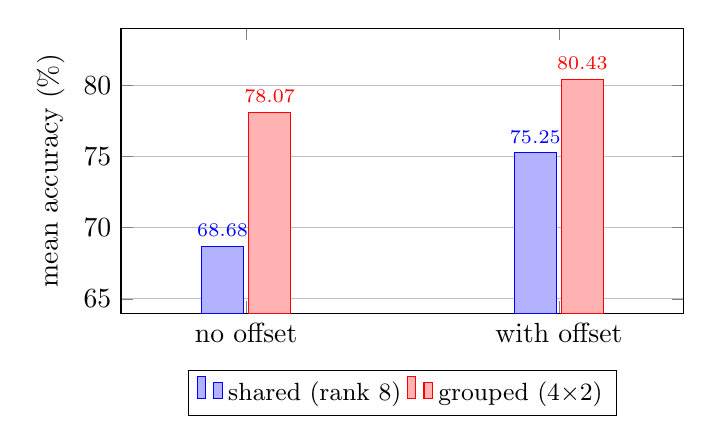
\begin{tikzpicture}
\begin{axis}[
  ybar, bar width=15pt,
  width=0.72\textwidth, height=5.2cm,
  enlarge x limits=0.4,
  ymin=64, ymax=84,
  ylabel={mean accuracy (\%)},
  symbolic x coords={no offset,with offset},
  xtick=data,
  nodes near coords, nodes near coords style={font=\scriptsize},
  legend style={at={(0.5,-0.20)},anchor=north,legend columns=2,font=\small},
  ymajorgrids, tick align=inside,
]
\addplot coordinates {(no offset,68.68) (with offset,75.25)};
\addplot coordinates {(no offset,78.07) (with offset,80.43)};
\legend{shared (rank $8$),grouped ($4{\times}2$)}
\end{axis}
\end{tikzpicture}
\caption{The two capacity moves compose at a bit-identical budget. Bars are 3-seed
mean balanced accuracy (\%) over the $12$ scorable tasks for the four corners of the
$2\times2$ (Section~\ref{sec:method}); ``with offset'' is the per-scope offset. The
proposed grouped/offset cell ($80.43$) is best on every seed, and the end-to-end
gain over the standard shared/no-offset baseline ($68.68$) is $\mathbf{+11.76}$~pp.
Family routing and the offset are scored at their upper bounds
(Section~\ref{sec:limitations}).}
\label{fig:combined-2x2}
\end{figure}

\begin{table}[t]
\centering
\small
\caption{The $2\times2$ decomposed into its four effects (3-seed means, per-seed in
brackets). Every effect is positive on all three seeds, so the two moves are
independent and additive. The grouping-alone effect here ($+9.39$~pp) is the
no-offset column of \emph{this} offset-arm run, a different arm set from the
standalone grouping experiment of Table~\ref{tab:grouping-alone} ($+8.00$~pp); both
are positive on all seeds.}
\label{tab:combined-effects}
\begin{tabular}{llc}
\toprule
effect & mean & per-seed / sign \\
\midrule
offset alone \ $(R_{\mathrm{sh{+}off}}-R_{\mathrm{sh}})$      & $+6.58$ & $+3.76,+5.29,+10.68$ \ all$+$ \\
grouping alone \ $(R_{\mathrm{gp}}-R_{\mathrm{sh}})$          & $+9.39$ & $+9.01,+8.34,+10.83$ \ all$+$ \\
grouping on top of offset \ $(R_{\mathrm{gp{+}off}}-R_{\mathrm{sh{+}off}})$ & $+5.18$ & $+6.82,+5.88,+2.84$ \ all$+$ \\
end-to-end \ $(R_{\mathrm{gp{+}off}}-R_{\mathrm{sh}})$        & $\mathbf{+11.76}$ & $+10.58,+11.18,+13.51$ \ all$+$ \\
\bottomrule
\end{tabular}
\end{table}

\noindent The proposed grouped/offset cell is best on every seed, and the two moves
are independent: grouping still adds $+5.18$~pp after the output layer is already
corrected, and the offset still adds on top of grouping, so neither subsumes the
other. The end-to-end $+11.76$~pp over the standard shared/no-offset baseline is
positive on all three seeds and roughly nine times the noise floor. This is the
paper's central positive claim: at a fixed parameter budget the two capacity
constraints of Section~\ref{sec:setup} are separately relievable and the relief adds.

\paragraph{Where the offset does \emph{not} add, stated plainly.}
The composition is not uniform across tasks, and the pattern is the expected one. The
representation gain from grouping-on-top-of-offset is concentrated on the tasks a
shared adapter had overwritten --- MNLI $+19.8$, QQP $+14.1$, RTE $+13.0$, SST-2
$+6.3$ (3-seed means of $R_{\mathrm{gp{+}off}}-R_{\mathrm{sh{+}off}}$) --- while on the
high-cardinality topic tasks the shared adapter's larger rank makes its offset-cell
competitive: DBpedia is $-0.5$ and WiC $-3.7$ under grouping. These are the same tasks
that lose in the grouping-alone breakdown and for the same reason, rank $2$ is too
small for a $14$-way label set. The net is decisively positive because the reused-token
families dominate the mean, but we report the topic-family cost rather than hide it,
and it is the concrete motivation for the adaptive per-family rank we leave to future
work.

\paragraph{Grouping de-stales the stored offset, turning its column deployable.}
The offset column above is fit against the \emph{final} model (the rehearsal ceiling
of Section~\ref{sec:sso}), an upper bound. The deployable rule fits each task's optimum
at the moment it finishes training, stores it, and never re-reads old data --- which
pays a staleness cost because the model keeps moving afterward. Section~\ref{sec:method}
argued that grouping should soften this: a family adapter is perturbed only by its own
family's later tasks, so a stored per-family optimum drifts less than one stored against
a monolithic adapter that every later task moves. We now measure it. Holding the
Chebyshev aggregation ($m{=}1$), the scope routing, and the scored \texttt{audit} split
identical, we compare the stored offset (fit at each task's boundary) against the refit
upper bound (fit against the final model); only the fit \emph{time} differs, so the gap
$\text{staleness}=R_{\mathrm{refit}}-R_{\mathrm{stored}}$ is pure staleness
(Figure~\ref{fig:destale}).

\begin{figure}[t]
\centering
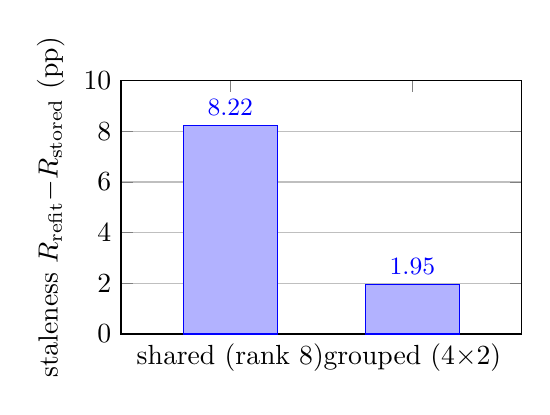
\begin{tikzpicture}
\begin{axis}[
  ybar, bar width=34pt,
  width=0.55\textwidth, height=4.8cm,
  enlarge x limits=0.6,
  ymin=0, ymax=10,
  ylabel={staleness $R_{\mathrm{refit}}{-}R_{\mathrm{stored}}$ (pp)},
  symbolic x coords={shared (rank 8),grouped ($4{\times}2$)},
  xtick=data,
  nodes near coords, nodes near coords style={font=\small},
  ymajorgrids, tick align=inside,
]
\addplot coordinates {(shared (rank 8),8.22) (grouped ($4{\times}2$),1.95)};
\end{axis}
\end{tikzpicture}
\caption{Grouping de-stales the stored offset. Bars are 3-seed mean staleness
$R_{\mathrm{refit}}-R_{\mathrm{stored}}$ (pp), holding the Chebyshev aggregation,
scope routing, and \texttt{audit} split fixed so only fit \emph{time} differs.
Grouping cuts staleness from $8.22$~pp (per-seed $7.98,10.08,6.62$) to $1.95$~pp
($1.16,3.88,0.82$): a $+6.27$~pp reduction, positive on all three seeds. The stored
offset's net gain over no offset remains mixed in sign (see text).}
\label{fig:destale}
\end{figure}

\noindent Grouping cuts the staleness of the deployable stored offset from $8.22$~pp to
$1.95$~pp, positive on all three seeds with small variance: under the grouped allocation
the deployable stored offset recovers all but $\sim2$~pp of the refit upper bound, where
on a shared adapter it forfeits over $8$~pp. This is the mechanism of
Section~\ref{sec:method} confirmed directly, and it is what lets the offset column of the
$2\times2$ be read as (near-)deployable rather than only as a ceiling. We state one
limit plainly: the stored offset's \emph{net} gain over no offset ($R_{\mathrm{stored}}-
R_{\mathrm{none}}$) is $-0.51$~pp mean under grouping and mixed in sign across seeds
($+0.14,-1.67,+0.02$), against $-1.95$~pp on the shared adapter. So grouping removes the
staleness \emph{penalty} that made the stored offset actively harmful on a shared adapter
(Section~\ref{sec:sso}'s $-5.08$~pp), but it does not, on this stream, make the deployable
offset a reliable net \emph{gain} on its own --- its value is that it now tracks the
upper-bound offset the composed method uses, closing most of the deployment gap that
Section~\ref{sec:limitations} had flagged.

\section{Limitations}
\label{sec:limitations}

\paragraph{One stream, one order, one model.}
Every number here comes from a single task order (Order-4) on a single backbone
(T5-large, LoRA $r{=}8$ on $q/v$) at a single budget ($400$/class, $3$ epochs).
Order effects in continual learning are large, and we have not measured them. The
scope structure that drives the whole analysis is a property of \emph{this}
benchmark: ten of fifteen tasks share output tokens. A stream whose tasks have
pairwise disjoint verbalizers has $\Delta^{\mathrm{id}}\equiv0$ by
Proposition~\ref{prop:disjoint}, and on such a stream nothing in this paper
applies. We regard the direction of that dependence as the honest framing: we
identify a term that exists when verbalizers are shared, and we say so rather than
implying generality.

\paragraph{The theory is proved in a special case that happens to cover us.}
Proposition~\ref{prop:qm} is proved for $d=1$ --- binary shared verbalizers --- and
for any $m$. The case $m\ge2$ with dimension $\ge2$ is \textbf{open}. It happens
that every scorable multi-task scope on this stream is binary, so every $q_m$ we
report is backed by proof; but that is a fact about which tasks survived our
exclusion rules, not a fact about the theory. A stream with scorable $K_S\ge3$
shared scopes would take us outside what we have proved.

\paragraph{The accuracy-space bound is weak where it matters.}
Proposition~\ref{prop:cheb-acc} carries a measured constant
$\kappa\approx0.018$ (worst task, WiC). At that value the bound is not
practically informative, and we do not rest any empirical claim on it: the
unconditional geometric statement does the work, and the accuracy numbers are
measured. Two conservatisms remain unresolved --- multi-class flip fractions count
only top-$2$ flips, and these $\kappa$ were estimated from an under-trained run
rather than re-estimated after convergence.

\paragraph{Three failed interventions are not a proof that none can work.}
Section~\ref{sec:three-anchors} reports that an orthogonality penalty of O-LoRA's
form, verbalizer-logit anchoring, and gauge-fixed anchoring all failed to improve
task-agnostic accuracy, two of them harmfully. The reading we prefer --- that the
identification gap is not a parameter-space object --- is an inference, not a
theorem. The alternative reading is that better parameter-space interventions exist
and we did not find them, and nothing in our evidence excludes it. We also tested
exactly one $\lambda$ grid per intervention, selected on a $6$-task prefix; in the
GFA case that gate demonstrably failed to predict $15$-task behaviour, which is a
weakness of our selection procedure and not only of the method.

\paragraph{Our two sensitivity analyses are underpowered, and we say so with numbers.}
Section~\ref{sec:sso} reports that neither the scale dependence of
$\Delta^{\mathrm{id}}$ nor the growth of staleness with stream length is established
here, and the design explains why. Live scope membership only ever takes the values
$\{1,2,3,4\}$, and only two scopes ever exceed one member, so task identity and
membership count cannot be fully separated; membership is also monotone in stage, so
``more scope-mates'' and ``later in the stream'' are collinear by construction. On
the staleness side, five scorable singleton tasks are trained at positions
$4,7,12,13,15$, giving age spans $0..11$, $0..8$, $0..3$, $0..2$ and $0..0$, so every
observation at age $\ge9$ comes from COPA alone. These are the reasons a failed
criterion here is weak evidence of absence rather than evidence of no effect, and
they were written down before the analysis was run.

\paragraph{Two of our four sensitivity arms are the same training trajectory.}
We had described Phase-2K and Phase-2P as two independent \texttt{none} arms for that
analysis. They are not: comparing their per-stage records field by field, all $480$
retention values agree \emph{bit for bit}, with identical gradient-step sequences and
identical seed, learning rate and epoch settings --- Phase-2P is Phase-2K's trajectory
with SSO scoring attached and its penalty weights at zero. The arm-invariance check is
therefore over one \texttt{none} replication (Phase-2Q) plus one different arm
(Phase-2M at $\lambda_a=0.5$), not three independent draws. The signs do agree across
all of them, but the check is weaker than we had claimed and we report it at the
corrected strength.

\paragraph{The enumeration is exhaustive only over its own constraint set.}
Section~\ref{sec:enumeration} claims exactly two non-vacuous admissible rules, and
that claim is an exhaustive case split over a table we wrote --- which examples a
rule may read and which model it may read them under. It is not a theorem about
task-agnostic inference. Three ways past it that our evidence does not close:
a rule that changes the training objective (our three anchors are three points in
that space, not a covering of it); a \emph{per-example} rather than per-task
router, which Section~\ref{sec:theory} shows can exceed even the per-task oracle
and whose task-free achievability we do not know; and stored state that is not an
estimate of a per-task optimum at all, for which our staleness mechanism gives no
prediction. ``Closed'' throughout this paper should be read as \emph{closed as
enumerated}, and the enumeration's premises are stated so they can be rejected.

\paragraph{Our O-LoRA arm is a re-implementation.}
The orthogonality penalty is our implementation of O-LoRA's regulariser inside our
harness at our budget. It is not the authors' code and not a reproduction of their
reported numbers. No comparison against their published table is made or implied,
and the arm exists to test additivity, not to benchmark.

\paragraph{The additivity question is unresolved, by our own criterion.}
Phase-2L's criterion C --- that the regulariser measurably repair deep forgetting on
the $>8$~pp stratum --- failed at both $\lambda$ values its gate selected. Our frozen
protocol says that when C fails, the additivity criteria A and B are
\emph{uninterpretable}. So we do not know whether an output-layer fix is additive
on top of a working representation-level method; we know only that it survived
alongside a penalty that did not measurably work. This is the single largest gap in
the paper's argument and we prefer to state it as such.

\paragraph{No comparison against published continual-PEFT methods.}
We did not run E$^2$-LoRA, NSR, LiteLoRA, SLICE, or ProCL. Every comparison here is
internal: arms differing in one component under an identical budget, identical
splits, and identical seeds. A claim that our approach outperforms published methods
would require running them, and we make no such claim.

\paragraph{Held-out data discipline costs us a number.}
The official test files are never opened. Everything is measured on \texttt{audit}
splits carved from training files, with offsets fit on disjoint \texttt{risk}
splits. This keeps the test sets clean for future work but means our absolute
accuracies are not comparable to published leaderboard numbers, and we do not place
them in such tables.

\paragraph{Our evaluation splits are class-balanced, and we measured what that buys
only once.}
Every \texttt{audit} split is $64$/class. Section~\ref{sec:bpo} shows this is not a
neutral choice: a rule that equalises predicted class frequencies gains $+4.40$~pp
on such a split and $-0.67$~pp at a $70{:}30$ mix. We pre-registered that control
for the query-batch rule because that rule's mechanism made the confound obvious.
\textbf{We did not run the equivalent control on anything else.} In particular the
$+1.51$~pp per-scope offset gain --- the paper's central measurement --- is a
balanced-split number, and while a per-scope offset fitted on labelled data has no
comparable reason to depend on query balance, we have not measured that it does not.
A reader should treat every accuracy in this paper as conditional on balanced
evaluation, and the one place we probed that condition, it mattered enough to change
a sign.

\paragraph{One frozen criterion could not be evaluated as written.}
Phase-2Q's protocol named a quantity its harness never recorded, so the criterion
guarding Proposition~\ref{prop:disjoint}'s wiring was unevaluable as frozen and we
reconstructed it --- correctly, and matching a formula already committed in an
earlier phase's decision script, but \emph{after} the phase's primary number was
known. We record it as unevaluable rather than passed, and the underlying prediction
is separately confirmed at $0/87$ by two other phases' checks. The general lesson is
against us: a pre-registration is only as strong as the harness that has to feed it,
and one of ours had a criterion that could never have fired. Our released notes
carry this and three other corrections to claims of our own, unedited beside the
appends that supersede them.

\paragraph{Excluded tasks.}
Three of fifteen tasks are excluded from scored means --- CB (rarest class $16$
examples, below the $40$ a $64$/class risk-plus-audit split needs), Yelp and Amazon
(five-way verbalizers sharing first sub-word pieces). The exclusions were fixed
before scoring and are the same in every arm, but they remove exactly the
higher-$K_S$ scopes, which is also where the open part of
Proposition~\ref{prop:qm} lives. A reader should treat our evidence as concerning
binary shared verbalizers.

\paragraph{Router state is not free, and we do not fold it into our headline cost.}
The $m{=}1$ table costs $33$ floats. Any $m>1$ variant additionally needs a
task-free router with per-task state that this figure does not cover; we report
that separately and never inside the same number.

\paragraph{Our proposed method is scored at two upper bounds.}
The combined method of Section~\ref{sec:combined} is measured with oracle scope
routing --- at evaluation we set each query's family adapter from its scope --- and
with the offset fit against the final model on each task's \texttt{risk} split. Both
are upper bounds, not deployable rules. A deployable system needs a task-free router
that recovers the family from the input alone; Section~\ref{sec:gap-real}'s honest
prototype router (nearest stored class-mean in encoder state) is the natural
candidate, and closing the grouped-oracle-to-grouped-routed gap is the first
measurement we owe. The $+11.76$~pp end-to-end number should therefore be read as the
achievable ceiling of the allocation, and a reviewer is entitled to discount it until
the router is measured. What is \emph{not} an upper bound is the fixed-budget
allocation itself: the four cells of the $2\times2$ share a bit-identical trainable
budget, so the comparison between them is exact regardless of routing.

\paragraph{Grouping de-stales the stored offset, but the deployable offset is not a net gain on its own.}
Section~\ref{sec:method} argued that a per-family adapter is perturbed only by its own
family, so a stored per-family offset should drift less than one stored against a
monolithic adapter. We measured this (Section~\ref{sec:combined}): grouping cuts the
staleness of the deployable stored offset from $8.22$~pp to $1.95$~pp, on all three
seeds, so the stored offset now tracks the refit upper bound the composed method reports.
Two honest limits remain. First, the offset column of the $2\times2$ is still \emph{run}
with the refit offset, not the stored one; we have shown the stored offset nearly matches
it, not re-run the whole $2\times2$ under the stored rule. Second, and more important, the
stored offset's net gain over no offset is $-0.51$~pp mean under grouping and mixed in
sign across seeds: grouping removes the active \emph{harm} that staleness caused on a
shared adapter ($-5.08$~pp in Section~\ref{sec:sso}), but on this stream it does not turn
the deployable offset into a reliable standalone improvement. The deployable value of the
offset is therefore that it composes with grouping at close to the upper bound, not that
it helps on its own.
\section{Conclusion}
\label{sec:conclusion}

Part of what looks like capacity exhaustion in continual PEFT is not, and the two
parts call for two different fixes. On a $15$-task stream under one fixed LoRA
adapter, an additive per-label offset on the verbalizer logits --- zero rank, a
handful of scalars --- recovers accuracy that rank-allocation methods are built to
protect; that is an \emph{output-layer} constraint. What the offset cannot recover
is the representation the shared adapter overwrote as later tasks arrived; that is a
distinct \emph{representation-layer} constraint. This paper measures both and
proposes a single fixed-budget method that relieves both: reallocate the rank across
task families so each family adapter drifts only under its own family, and add the
per-scope offset on top.

\emph{The two moves compose, at a bit-identical budget.} Splitting the tasks into
$K{=}4$ semantic families with a rank-$2$ adapter each --- exactly the parameters of
one shared rank-$8$ adapter --- beats the shared adapter by $+8.00$~pp across three
seeds. The per-scope offset adds $+6.58$~pp on its own, and still adds $+5.18$~pp on
top of grouping, so the two constraints are independent and neither fix subsumes the
other. End-to-end, the combined method beats the standard single-adapter baseline by
$+11.76$~pp, positive on every seed and roughly nine times the same-configuration
noise floor (Section~\ref{sec:combined}). The gain is a reallocation, not extra
capacity: the trainable-parameter count is bit-for-bit identical across all four
cells of the $2\times2$.

\emph{The output component is real and its information content is specific.} Under
one globally shared offset the identification gap is $3.13$~pp; under an offset
shared only within a verbalizer scope it is $0.00$~pp, CI $[-1.71,+1.71]$. Scope ---
free at inference, readable from the prompt --- recovers $+1.51$~pp, CI
$[+0.43,+2.74]$. The gap is exactly zero when verbalizer sets are disjoint
(Proposition~\ref{prop:disjoint}), which we verify in every run and which explains
why the per-task-head literature cannot see this term at all.

\emph{The objective is the wrong lever for the representation constraint.} An
orthogonality penalty of O-LoRA's form, verbalizer-logit anchoring, and gauge-fixed
anchoring all left task-agnostic accuracy unimproved, two of them harmfully. This is
what motivated changing the \emph{allocation} rather than the objective, and the
allocation move is what delivered the representation-layer gain the penalties could
not.

\paragraph{What we report at its upper bound, honestly.}
Both moves are scored at their upper bound: the offset is fit against the current
model and family routing uses the scope at evaluation. The deployable offset sources
each carry a measured cost on this stream. Storing per-task optima and applying the
scope's Chebyshev centre --- $33$ floats, no task index --- scores $5.08$~pp
\emph{below} using no offset at all, because a value fit at a task's boundary goes
stale as a monolithic adapter keeps moving; singleton scopes locate the cause with
aggregation, routing, and gauge ruled out by construction ($-4.18$~pp, CI
$[-6.61,-1.76]$). Computing the offset from the query batch instead gains $+4.40$~pp
and then inverts to $-0.67$~pp under the class-mix control we pre-registered against
our own balanced splits. We report both plainly. Grouping is positioned to soften
the staleness cost --- a per-family adapter drifts less than a monolithic one --- and
we mark the de-staling of stored offsets under grouping, and a task-free family
router, as the measurements that would close the deployment gap. Neither is claimed
here; the allocation result does not depend on them.

\paragraph{The one task that loses, and what it points to.}
The grouped allocation is not uniformly better. The $14$-way DBpedia loses $5.1$~pp
because rank $2$ is genuinely too small for it --- the only task negative in all three
seeds --- and it is the same task whose offset cell stays competitive under the
shared adapter's larger rank. We report it rather than average it away, and it is the
concrete motivation for an adaptive per-family rank: a topic family with fourteen
labels should draw more of the budget than a binary one. That is the natural next
rung, and unlike the offset-deployment questions it is a pure allocation question the
same method already frames.

\paragraph{Scope.}
One stream (Order-4), one backbone (T5-large), one budget (LoRA $r{=}8$, $2.36$M
trainable scalars), three seeds, generative PEFT with a shared decoder and
restricted-argmax scoring. Family routing and the offset are scored at their upper
bound, as stated. Every comparison is internal: arms differ in one component at an
identical budget with identical splits and seeds. We ran no published continual-PEFT
baseline and make no claim against one, and the official test files were never
opened, so our absolute accuracies do not belong in leaderboard tables. The budgeted
quantization result is proved for binary shared verbalizers and remains open beyond
them.


\section*{Reproducibility Statement}
We have tried to make every reported number retraceable to a frozen artefact
rather than to a description. The full protocol --- stream, splits, exclusion
rules, metrics, statistics, and the unconditional training gate --- is in
Appendix~\ref{app:experiments}, and the proofs with their exact hypotheses are in
Appendix~\ref{app:proofs}. The reference implementation, the harness, and the
decision scripts are released with the paper.

Each phase has a protocol file written before the run it governs, stating the
method, the criteria with numeric thresholds, and a set of predeclared outcomes
mapping possible results to conclusions; its SHA-256 is recorded on disk at freeze
time. Amendments are appended with their own date and hash, never edited in, so a
criterion cannot be restated once its result is known. The decision scripts are
frozen the same way, with thresholds as module-level constants and a constructed
failure case per criterion in their tests, so the map from numbers to verdicts
exists before the numbers do.

We state the limit of that scheme rather than implying a stronger form of
pre-registration than we have: the hashes pin the artefacts, and the ordering of
freeze and run rests on the committed source and the appended amendment record,
not on a timestamped external registry. No pre-run hash log survives for the
earliest phase, and we corrected an earlier sentence of ours that claimed
otherwise.

Six amendments in our record correct or retract claims of our own: a scope-class
split that did not survive bootstrapping; a headline result that an oracle-free
rerun collapsed; a $-5.66$~pp single-seed effect that vanished to $+0.28$~pp once
the remaining two seeds landed, which forced a wording change in
Section~\ref{sec:three-anchors}; a sentence asserting a state of our own code
that was not true when written, retracted the same day with the code then made to
match; an unmeasured claim that staleness grows with stream length, which we then
measured and could not establish, so the sentence was demoted in
Section~\ref{sec:sso}; and a description of two of our arms as independent
replications when a field-by-field comparison shows they are the same training
trajectory. All six remain in the released notes, unedited, beside the appends that
supersede them. Where a criterion failed we
report it under its own name, including one we had predicted would fail and one
that refuted our own proposed mechanism. All comparisons are internal: arms
differing in one component at identical budget, splits, and seeds. We run no
published continual-PEFT baseline and make no claim against one, and the official
test files are never opened, so our absolute accuracies are not comparable to
leaderboard numbers.

\section*{Large Language Model Usage Disclosure}
Large language model based agents were used extensively throughout this project,
well beyond copy-editing. Their contributions include: implementing and debugging
the experimental code and statistical harness; proposing and iterating on method
design, including the streamed offset table and the label-free inference rule;
proving and, in two cases, correctly narrowing the propositions of
Appendix~\ref{app:proofs};
running and interpreting the diagnostic and ablation analyses; drafting the
statistical procedure; and drafting, revising, and copy-editing the manuscript,
appendix, and protocol notes. The research direction, the honesty constraints, the
final scientific claims, and all go/no-go decisions were set and adjudicated by the
human authors. Every theoretical statement, every reported number, and every cited
reference was re-derived or re-checked against the underlying proofs, the frozen run
outputs, and the primary sources; the authors take full responsibility for all
content, including any errors introduced with model assistance. We flag this level
of assistance explicitly so that reviewers can weight the provenance of the design
and analysis accordingly.

\bibliography{references}
\bibliographystyle{iclr2026_conference}

\appendix
\section{Proofs}
\label{app:proofs}

This appendix proves the five propositions of the main text and states, for each,
exactly where the proof stops. Two of them are unconditional
(Propositions~\ref{prop:disjoint} and~\ref{prop:cheb}); two are conditional on a
margin-density constant $\kappa$ that we measure rather than assume
(Propositions~\ref{prop:cheb-acc} and~\ref{prop:amp}); one is proved in the
special case $d=1$ that covers every scorable multi-task scope on our benchmark
and is open beyond it (Proposition~\ref{prop:qm}). We also record, in
Appendix~\ref{app:narrowed}, three claims that earlier drafts of this work stated
too strongly, together with the counterexamples that forced the narrowing. They
are kept visible because each one changes how a number in the main text may be
reported.

\subsection{Setting and gauge}
\label{app:gauge}

Fix a scope $S$ with label set $Y_S=\{\ell_1,\dots,\ell_{K}\}$, $K=K_S$. For an
input $\bx$ and adapter parameters $\theta$, write the verbalizer-restricted logit
vector
\begin{equation}
  \bm{\lambda}_\theta(\bx)\in\R^{K},
  \qquad
  \big[\bm{\lambda}_\theta(\bx)\big]_k = \bu_{\ell_k}^\top\bh_\theta(\bx),
  \label{eq:app-logit}
\end{equation}
with $\bu_y$ the frozen unembedding row for token $y$. An offset $\bb\in\R^{K}$
acts by $\hat y(\bx)=\arg\max_k\big([\bm{\lambda}_\theta(\bx)]_k+b_k\big)$.

\paragraph{The gauge.}
For any $c\in\R$, the offsets $\bb$ and $\bb+c\mathbf{1}$ induce the same
restricted argmax at every input, so $\bb$ acts only through its image in the
quotient $\R^{K}/\mathrm{span}(\mathbf{1})$. We fix the gauge by the zero-sum
projector
\begin{equation}
  P_0\bb \;=\; \bb - \Big(\tfrac{1}{K}\textstyle\sum_k b_k\Big)\mathbf{1},
  \qquad
  V_0 \;=\; \{\bm{v}\in\R^{K}:\ \textstyle\sum_k v_k = 0\}\ \cong\ \R^{K-1},
  \label{eq:app-gauge}
\end{equation}
and equip $V_0$ with the Euclidean norm. Every offset below is an element of
$V_0$. This is the same $P_0$ as in Section~\ref{sec:method}, and it is the reason
Equation~\eqref{eq:cost} counts $K_S-1$ rather than $K_S$ scalars per stored
vector.

For $K=2$ the space $V_0$ is one-dimensional: $P_0\bb=(-t,t)$ with
$t=(b_1-b_0)/2$, so an offset is fully described by the scalar contrast
$s=b_1-b_0$, and $\|P_0\bb-P_0\bb'\|_2=|s-s'|/\sqrt2$. This constant $1/\sqrt2$ is
a unit convention, not a dimension: it is why a scope whose four member contrasts
span a range of exactly $2$ is recorded with $q_1=0.7071$.

Write $R_g(\bb)$ for task $g$'s balanced accuracy under shared offset $\bb$ at the
current parameters, and
\begin{equation}
  \bz_g \in \argmax_{\bm{v}\in V_0} R_g(\bm{v}),
  \qquad
  R_g^{\mathrm{orc}} = R_g(\bz_g).
  \label{eq:app-orc}
\end{equation}
Ties in \eqref{eq:app-orc} are broken by any fixed rule; nothing below depends on
which, because the statements quantify over all shared $\bb$ and refer to $\bz_g$
only through its gauge-fixed value.

\subsection{Proof of Proposition~\ref{prop:disjoint} (disjoint verbalizers give a zero gap)}
\label{app:proof-disjoint}

\begin{proof}
Suppose the verbalizer sets $Y_1,\dots,Y_T$ are pairwise disjoint. An offset in
the sense of Section~\ref{sec:setup} is a vector $\bb\in\R^{V}$ over the whole
vocabulary, and task $g$'s prediction reads only the coordinates $\{b_y:y\in Y_g\}$.
Let $\bb_g^\star\in\R^{V}$ be an optimal offset for task $g$, supported on $Y_g$
(any optimal offset may be restricted to $Y_g$ without changing $g$'s predictions,
since coordinates outside $Y_g$ never enter $g$'s argmax). Define
\begin{equation}
  \bb^\star \;=\; \sum_{g=1}^{T}\bb_g^\star .
  \label{eq:app-disjoint-sum}
\end{equation}
Because the supports are pairwise disjoint, for every $g$ and every $y\in Y_g$ we
have $b^\star_y = [\bb_g^\star]_y$. Hence the restricted argmax of task $g$ under
$\bb^\star$ agrees with its restricted argmax under $\bb_g^\star$ at every input,
so $R_g(\bb^\star)=R_g^{\mathrm{orc}}$ for all $g$ simultaneously. Since
$R_g^{\mathrm{shr}}$ is the accuracy under the \emph{best} single shared offset, it
is at least $R_g(\bb^\star)$, and it is at most $R_g^{\mathrm{orc}}$ always. Both
inequalities together give $R_g^{\mathrm{shr}}=R_g^{\mathrm{orc}}$ and therefore
$\Delta_g^{\mathrm{id}}=0$ for every $g$ and every time $t$.
\end{proof}

\begin{remark}[The singleton corollary we use as a wiring check]
\label{rem:singleton}
The same argument applied to a single scope gives the form used in
Section~\ref{sec:method}: if $|\mathrm{mem}(S)|=1$ then $Z_S$ is a one-point set,
its Chebyshev centre \emph{is} that point, and $r_S=0$ exactly. This is a
prediction of the theory with no free constant, so any nonzero measured
$\Delta^{\mathrm{id}}$ on a singleton scope is a bug rather than a finding, and we
report the check in every run ($0$ violations, $87$--$144$ observations per arm,
worst absolute deviation $0.0$). Note what the check does \emph{not} cover: it
constrains the scoped rung, not a stored-offset method, because a stored optimum
is fitted at an earlier parameter value. That distinction is exactly what makes
the singleton split of Section~\ref{sec:sso} an isolate for staleness.
\end{remark}

\begin{remark}[Why this is the honest boundary, not a weakness]
Proposition~\ref{prop:disjoint} says the phenomenon we study has a precondition
that is a property of the benchmark and is checkable without running anything: the
tasks must reuse output tokens. On a stream with pairwise disjoint verbalizers
$\Delta^{\mathrm{id}}\equiv0$ and nothing in this paper applies. We state it first
for that reason.
\end{remark}

\subsection{Proof of Proposition~\ref{prop:cheb} (logit-space minimax)}
\label{app:proof-cheb}

Recall $Z_S=\{P_0\bz_g : g\in\mathrm{mem}(S)\}\subset V_0$, a finite set of
$n=|\mathrm{mem}(S)|$ points, and
$F(\bb)=\max_{g\in\mathrm{mem}(S)}\|\bb-P_0\bz_g\|_2$.

\begin{proof}
\emph{(i) The minimum over $\R^{K}$ is attained inside $V_0$.}
For $\bb\in\R^{K}$ decompose $\bb = P_0\bb + \beta\mathbf{1}$ with
$\beta=\frac1K\sum_k b_k$. Since every $\bm{p}\in Z_S$ lies in $V_0$ and
$\mathbf{1}\perp V_0$, Pythagoras gives
$\|\bb-\bm{p}\|_2^2 = \|P_0\bb-\bm{p}\|_2^2 + K\beta^2 \ge \|P_0\bb-\bm{p}\|_2^2$,
with equality iff $\beta=0$. So $F(\bb)\ge F(P_0\bb)$ with equality iff
$\bb\in V_0$, and it suffices to minimise $F$ over $V_0$.

\emph{(ii) The minimum is attained.}
$F$ is a finite maximum of convex functions, hence convex, and continuous. It is
coercive: $F(\bb)\ge\|\bb\|_2-\max_g\|P_0\bz_g\|_2\to\infty$. A continuous coercive
function on the finite-dimensional space $V_0$ attains its infimum, and by
definition that infimum is the Chebyshev radius $r_S$ of $Z_S$ and its minimiser
set is the set of Chebyshev centres. This gives \eqref{eq:cheb}.

\emph{(iii) The minimiser is unique.}
Suppose $\bb_1\neq\bb_2$ both attain $F=r_S$, and let
$\bar\bb=\tfrac12(\bb_1+\bb_2)$. For each $\bm{p}\in Z_S$, the parallelogram law
applied to $\tfrac12(\bb_1-\bm{p})+\tfrac12(\bb_2-\bm{p})$ gives
\begin{equation}
  \|\bar\bb-\bm{p}\|_2^2
  \;=\;\tfrac12\|\bb_1-\bm{p}\|_2^2+\tfrac12\|\bb_2-\bm{p}\|_2^2
      -\tfrac14\|\bb_1-\bb_2\|_2^2
  \;\le\; r_S^2-\tfrac14\|\bb_1-\bb_2\|_2^2
  \;<\;r_S^2 .
  \label{eq:app-parallelogram}
\end{equation}
Taking the maximum over $\bm{p}\in Z_S$ yields $F(\bar\bb)<r_S$, contradicting
minimality. Hence the Chebyshev centre is unique. Combined with (i), the minimiser
over all of $\R^{K}$ is unique as well, and it is the zero-mean representative.

\emph{(iv) The diameter bound.}
For any $g,g'\in\mathrm{mem}(S)$ and any $\bb\in V_0$, the triangle inequality gives
$\|P_0\bz_g-P_0\bz_{g'}\|_2\le\|\bb-P_0\bz_g\|_2+\|\bb-P_0\bz_{g'}\|_2\le 2F(\bb)$.
Maximising the left side over the pair and minimising the right over $\bb$ gives
$r_S\ge\tfrac12\mathrm{diam}(Z_S)$. In particular $r_S=0$ iff
$\mathrm{diam}(Z_S)=0$, i.e.\ iff all member optima coincide after gauge fixing.

\emph{(v) $r_S=q_1(S)$.}
The $m$-centre quantization radius of Section~\ref{sec:ladder} is
$q_m(Z_S)=\min_{|C|\le m}\max_{\bm{p}\in Z_S}\mathrm{dist}(\bm{p},C)$. At $m=1$ a
codebook is a single point $C=\{\bb\}$ and $\mathrm{dist}(\bm{p},C)=\|\bb-\bm{p}\|_2$,
so $q_1(Z_S)=\min_{\bb} F(\bb)=r_S$.
\end{proof}

\begin{remark}[Uniqueness is a statement about vectors, not about decision rules]
Part (iii) gives a unique minimising \emph{vector} in $V_0$. As an inference rule
the minimiser is unique only modulo $\mathrm{span}(\mathbf{1})$, by the gauge
freedom of Appendix~\ref{app:gauge}; the zero-mean representative is the
norm-minimal member of that equivalence class. This is why the method stores
$P_0\bz_g$ and not $\bz_g$, and why the cost \eqref{eq:cost} is $K_S-1$ per vector.
\end{remark}

\begin{remark}[What makes the target streamable]
\label{rem:streamable}
The right-hand side of \eqref{eq:cheb} is a function of the member optima $Z_S$
alone. It does not involve the members' examples, their logits, their sample sizes,
or their arrival order. That is the entire licence for the method of
Section~\ref{sec:method}: if the target depended on the data through anything more
than $Z_S$, storing a $K_S$-vector per task could not in principle suffice.
Proposition~\ref{prop:cheb} therefore establishes that the SSO \emph{target} is
representable at the stated cost --- and nothing more. It does not establish that
the stored vectors remain valid as $\theta$ moves, which is the empirical question
Section~\ref{sec:sso} answers in the negative.
\end{remark}

\subsection{Proposition~\ref{prop:cheb-acc}: from distance to accuracy, and what it costs}
\label{app:proof-cheb-acc}

Proposition~\ref{prop:cheb} bounds a \emph{distance}. Turning it into a statement
about accuracy requires an assumption, and the reason is not technical: a distance
can be large while costing nothing. If every example of every member task sits far
from its decision boundary, moving the shared offset by a bounded amount flips no
prediction and each $R_g$ is locally constant. We therefore separate two
quantities that an earlier draft of this work conflated.

\begin{definition}[Disagreement and accuracy-decay profiles]
\label{def:profiles}
Fix a task $g$ and let $\hat y(\cdot\,;\bb)$ denote its restricted argmax under
offset $\bb$. For $t\ge0$ define
\begin{align}
  \Phi_g(t) &= \min_{\bm{u}\in V_0,\ \|\bm{u}\|_2=1}
    \ \Pr_{\bx\sim\cD_g}\!\big[\hat y(\bx;\bz_g+t\bm{u})\neq \hat y(\bx;\bz_g)\big],
    \label{eq:app-phi}\\
  \Psi_g(t) &= \min_{\bm{u}\in V_0,\ \|\bm{u}\|_2=1}
    \ \big[R_g(\bz_g)-R_g(\bz_g+t\bm{u})\big].
    \label{eq:app-psi}
\end{align}
$\Phi_g$ is the smallest fraction of predictions that \emph{change} when the offset
is displaced a distance $t$ from $g$'s own optimum; $\Psi_g$ is the smallest
resulting \emph{loss of accuracy}. Both minima are over directions, so both are
worst-case over the direction the shared offset happens to lie in. By optimality
of $\bz_g$ in \eqref{eq:app-orc}, $\Psi_g(t)\ge0$ for all $t$.
\end{definition}

\begin{assumption}[Margin density, disagreement form]
\label{asm:kappa-dis}
There exist $\kappa_{\mathrm{dis}}>0$ and $t_0>0$ with
$\Phi_g(t)\ \ge\ \kappa_{\mathrm{dis}}\cdot\min(t,t_0)$ for every $t\ge0$ and every
$g\in\mathrm{mem}(S)$.
\end{assumption}

\begin{assumption}[Margin density, accuracy form]
\label{asm:kappa-acc}
There exist $\kappa>0$ and $t_0>0$ with
$\Psi_g(t)\ \ge\ \kappa\cdot\min(t,t_0)$ for every $t\ge0$ and every
$g\in\mathrm{mem}(S)$.
\end{assumption}

Assumption~\ref{asm:kappa-acc} is the hypothesis of
Proposition~\ref{prop:cheb-acc} as stated in Section~\ref{sec:theory}; the
interval $[0,\varepsilon]$ there is $[0,t_0]$ here. The proof is then two lines,
and this is deliberate: the work is done by \emph{where} the two statements live,
not by the inequality itself.

\begin{proof}[Proof of Proposition~\ref{prop:cheb-acc}]
Let $\bb\in V_0$ be any shared offset on $S$. By Proposition~\ref{prop:cheb} there
is a member $g$ with $t:=\|\bb-P_0\bz_g\|_2\ \ge\ r_S$. Set
$\bm{u}=(\bb-P_0\bz_g)/t$ if $t>0$ (if $t=0$ then $r_S=0$ and the claim is
vacuous). Since $\Psi_g$ minimises over unit directions,
\begin{equation}
  R_g^{\mathrm{orc}}-R_g(\bb)
  \;=\; R_g(\bz_g)-R_g(\bz_g+t\bm{u})
  \;\ge\; \Psi_g(t)
  \;\ge\; \kappa\min(t,t_0)
  \;\ge\; \kappa\min(r_S,t_0),
  \label{eq:app-cheb-acc-chain}
\end{equation}
using Assumption~\ref{asm:kappa-acc} and then $t\ge r_S$ together with
monotonicity of $\tau\mapsto\min(\tau,t_0)$. Taking the maximum over
$g\in\mathrm{mem}(S)$ on the left can only increase it, which is
\eqref{eq:cheb-acc}.
\end{proof}

\noindent The same argument with $\Phi$ in place of $\Psi$ gives the disagreement
form, which we record separately because it is the one our measurement certifies.

\begin{lemma}[Disagreement-space minimax]
\label{lem:dis-minimax}
Under Assumption~\ref{asm:kappa-dis}, for every shared $\bb$ on $S$,
\begin{equation}
  \max_{g\in\mathrm{mem}(S)}
    \Pr_{\bx\sim\cD_g}\!\big[\hat y(\bx;\bb)\neq\hat y(\bx;\bz_g)\big]
  \;\ge\; \kappa_{\mathrm{dis}}\cdot\min(r_S,t_0).
\end{equation}
\end{lemma}

\subsubsection{What the measured constant certifies, stated precisely}
\label{app:kappa-measured}

We report $\kappa\approx0.0182$ (worst task, WiC) in Section~\ref{sec:theory}. The
estimator behind that number is a top-$2$ margin CDF, so it estimates
$\kappa_{\mathrm{dis}}$ of Assumption~\ref{asm:kappa-dis}, not $\kappa$ of
Assumption~\ref{asm:kappa-acc}. The two are ordered, and only in one direction:

\begin{lemma}[The disagreement constant bounds the accuracy constant]
\label{lem:kappa-order}
$\Psi_g(t)\le\Phi_g(t)$ for all $t\ge0$. Consequently the largest valid constant in
Assumption~\ref{asm:kappa-acc} is at most the largest valid constant in
Assumption~\ref{asm:kappa-dis}: $\kappa\le\kappa_{\mathrm{dis}}$.
\end{lemma}

\begin{proof}
Fix $g$ and $t$, and for a unit direction $\bm{u}$ write
$\Psi_g^{\bm{u}}(t)=R_g(\bz_g)-R_g(\bz_g+t\bm{u})$ and
$D_g^{\bm{u}}(t)=\Pr[\hat y(\bx;\bz_g+t\bm{u})\neq\hat y(\bx;\bz_g)]$.

\emph{Step 1 (pointwise in $\bm{u}$).} Let $A$ be the event that the prediction is
correct at $\bz_g$ and incorrect at $\bz_g+t\bm{u}$, and $B$ the reverse. Then
$\Psi_g^{\bm{u}}(t)=\Pr[A]-\Pr[B]\le\Pr[A]\le\Pr[A\cup B]\le D_g^{\bm{u}}(t)$,
since $A$ and $B$ are disjoint subsets of the disagreement event.

\emph{Step 2 (transfer to the profiles).} Let $\bm{u}^\star$ attain
$\Phi_g(t)=\min_{\bm{u}}D_g^{\bm{u}}(t)$, which exists because the unit sphere in
$V_0$ is compact and $D_g^{\bm{u}}$ takes finitely many values on a finite sample.
Then
\begin{equation}
  \Psi_g(t)\;=\;\min_{\bm{u}}\Psi_g^{\bm{u}}(t)
  \;\le\;\Psi_g^{\bm{u}^\star}(t)
  \;\le\;D_g^{\bm{u}^\star}(t)
  \;=\;\Phi_g(t).
\end{equation}

\emph{Step 3.} If Assumption~\ref{asm:kappa-acc} holds with constant $\kappa$ then
$\kappa\min(t,t_0)\le\Psi_g(t)\le\Phi_g(t)$, so Assumption~\ref{asm:kappa-dis}
holds with the same constant. Hence the supremum of valid $\kappa$ is no larger
than the supremum of valid $\kappa_{\mathrm{dis}}$.
\end{proof}

\noindent So the number we measured is an \emph{upper} estimate of the constant that
Proposition~\ref{prop:cheb-acc} needs. We state the consequence rather than leaving
it implicit: \textbf{Equation~\eqref{eq:cheb-acc} evaluated at
$\kappa=0.0182$ is an optimistic reading of a bound we have not separately
certified, and Lemma~\ref{lem:dis-minimax} at
$\kappa_{\mathrm{dis}}=0.0182$ is the statement our measurement supports.} Nothing
downstream changes, because no empirical claim in this paper is derived from
\eqref{eq:cheb-acc}: the geometric half carries the load and every accuracy-space
number we report is measured. But the distinction has to be on the page, because
$0.0182$ appears next to an accuracy-space inequality in the main text.

Three further gaps between the assumption and the estimator, in the order they
matter:

\begin{enumerate}
  \item \textbf{Centring.} The estimator computes the margin CDF of the raw
    verbalizer logits, i.e.\ the flip curve around $\bb=\mathbf{0}$, whereas
    Definition~\ref{def:profiles} centres at $\bz_g$. The two differ by a shift of
    the margin distribution and \emph{we do not know the sign of the discrepancy};
    it is a proxy, not a conservative one.
  \item \textbf{Grid safety.} The curve is recorded on
    $t\in\{0.1,0.25,0.5,1,1.5,2,3,4\}$. The naive slope $\min_i N(t_i)/t_i$
    verifies $N(t)\ge\kappa t$ only at grid points, while the assumption needs all
    $t$; since $N$ is non-decreasing the worst case in $[t_i,t_{i+1})$ is
    $t\to t_{i+1}^-$ with $N$ still at $N(t_i)$, so the valid slope is
    $\min_i N(t_i)/t_{i+1}$. Grid ratios reach $2.5\times$ and the two columns
    differ by up to that factor. Only the latter is a lower bound, and it is what
    we report.
  \item \textbf{Multi-class conservatism.} For $K_S\ge3$ only top-$2$ flips are
    counted, so $N$ is itself a lower bound on the flip fraction and
    $\kappa_{\mathrm{dis}}$ is understated for MNLI, AGNews, DBpedia, Yahoo, Yelp
    and Amazon. This gap favours the bound.
\end{enumerate}

\noindent Item 2 is why the reported worst-task value is $0.0182$ rather than the
naive $0.0312$ or the older two-quantile estimate $0.0871$; the last should not be
cited. We quote the worst task rather than the median $0.0625$ because $\kappa$ must
hold \emph{simultaneously} for every member of a scope, so the smallest-$\kappa$
member sets the bound --- a median would overstate the usable constant by
$3.4\times$.

\subsubsection{The assumption is necessary, not decorative}
\label{app:kappa-necessary}

\begin{proposition}[No assumption-free accuracy-space form exists]
\label{prop:no-free-lunch}
There is no function $\omega$ with $\omega(\rho)>0$ for $\rho>0$ such that
$\max_{g\in\mathrm{mem}(S)}[R_g^{\mathrm{orc}}-R_g(\bb)]\ge\omega(r_S)$ holds for
every scope, every model and every shared $\bb$.
\end{proposition}

\begin{proof}
Two tasks share the binary verbalizer $\{\ell_0,\ell_1\}$, so $V_0\cong\R$ and an
offset is the scalar contrast $s$. Let task $1$ have every example at logit gap
$+c$ in favour of its true label and task $2$ every example at gap $-c$, for a
constant $c>0$. Then $z_1=0$ and any $z_2>c$ is optimal for task $2$, so
$r_S\ge c/2$. At $\bb=0$ task $1$ is perfect and task $2$ scores $0$, so the
left-hand side equals $1$ --- but it equals $1$ for \emph{every} $c$, including
$c\to0$, where $r_S\to0$. Conversely rescaling all logits by $\alpha$ multiplies
$r_S$ by $\alpha$ while leaving every argmax, hence every accuracy, unchanged. So
the left-hand side is constant along a family on which $r_S$ ranges over
$(0,\infty)$, and no positive $\omega(r_S)$ can bound it below for all members of
the family; taking $\alpha$ large also shows no upper bound of the form
$\omega(r_S)\le$ accuracy loss can be non-vacuous, since accuracy differences are
at most $1$ and $r_S$ is unbounded.
\end{proof}

\noindent This is the concrete form of the correction recorded in
Section~\ref{sec:theory}: an earlier version of our own analysis bounded an
accuracy difference below by a diameter-type quantity. Accuracy differences are at
most $1$; diameters are unbounded; the two are not comparable without a constant
that ties logit distance to flip probability. That constant is $\kappa$, and
Proposition~\ref{prop:no-free-lunch} is why it cannot be removed.

\begin{remark}[What the conditional proposition is still worth]
Given how close Assumption~\ref{asm:kappa-acc} is to the conclusion of
Proposition~\ref{prop:cheb-acc}, it is fair to ask what the proposition adds. The
answer is a change of quantifier, not a strengthening of the rate. The assumption
is \emph{local}, \emph{per-task}, and about a single task's own neighbourhood; the
conclusion is about the \emph{worst member of a scope} and its right-hand side
$r_S$ is a function of the member optima alone --- computable, by
Proposition~\ref{prop:cheb}, from the geometry of the demands without reference to
any model or dataset. That transfer is the content. We do not claim more for it,
and at $\kappa\approx0.018$ we do not use it quantitatively.
\end{remark}

\subsection{Proof of Proposition~\ref{prop:qm} (budgeted offsets)}
\label{app:proof-qm}

A budget of $m$ task-free offsets on a scope is a \emph{codebook}
$C=\{\bm{c}_1,\dots,\bm{c}_m\}\subset V_0$ together with a rule assigning each task
to a centre. Write $X=Z_S\subset V_0$ for the member optima, $d=\dim V_0=K_S-1$,
$T=|X|$, and
\begin{equation}
  q_m(X)\;=\;\min_{|C|\le m}\ \max_{\bm{x}\in X}\ \mathrm{dist}(\bm{x},C),
  \qquad \mathrm{dist}(\bm{x},C)=\min_{j}\|\bm{x}-\bm{c}_j\|_2 .
  \label{eq:app-qm}
\end{equation}
By construction $q_1\ge q_2\ge\cdots\ge q_T=0$, which is the monotonicity of the
ladder in Section~\ref{sec:ladder}. Note that \eqref{eq:app-qm} presumes
nearest-centre assignment; a task-free router that assigns otherwise can only do
worse, which is why $q_m$ is a bound on any routed method and not a promise about
one.

\subsubsection{The closed form at \texorpdfstring{$d=1$}{d=1}}

\begin{proposition}[Closed form, $m=2$, $d=1$]
\label{prop:q2-closed}
Let $X=\{x_1\le\cdots\le x_T\}\subset\R$ with $T\ge2$. Then
\begin{equation}
  q_2(X)\;=\;\min_{1\le j\le T-1}\ \max\!\Big(\tfrac{x_j-x_1}{2},\ \tfrac{x_T-x_{j+1}}{2}\Big),
  \label{eq:app-q2}
\end{equation}
attained by $C=\{\tfrac{x_1+x_j}{2},\ \tfrac{x_{j+1}+x_T}{2}\}$ for a minimising $j$.
\end{proposition}

\begin{proof}
\emph{Step 1: an optimal $2$-codebook induces a contiguous split.} Let
$C=\{c_1\le c_2\}$ and assign each point to its nearest centre. In $\R$ the
nearest-centre rule assigns $x$ to $c_1$ iff $x\le(c_1+c_2)/2$, so the assignment
is a threshold rule: there is $j\in\{0,\dots,T\}$ with $\{x_1,\dots,x_j\}\to c_1$
and $\{x_{j+1},\dots,x_T\}\to c_2$. Only the $T+1$ contiguous splits need be
considered. This is exactly the step that fails for $d\ge2$: there the Voronoi
cells of two centres are half-spaces, but enumerating orderings of the points does
not enumerate the achievable bipartitions.

\emph{Step 2: within a block the best centre is the midrange.} For a finite
$B\subset\R$, $\min_c\max_{x\in B}|x-c|=(\max B-\min B)/2$, attained uniquely at
$c=(\max B+\min B)/2$: for any $c$,
$\max_{x\in B}|x-c|\ge\tfrac12[(\max B-c)+(c-\min B)]=(\max B-\min B)/2$, with
equality iff $c$ is the midpoint.

\emph{Step 3: combine.} For split $j$ the covering radius is
$\max\big((x_j-x_1)/2,(x_T-x_{j+1})/2\big)$ by Step 2 applied to each block.
Minimising over $j$ gives \eqref{eq:app-q2}. The degenerate splits $j=0$ and $j=T$
leave one block empty and reduce to $q_1=(x_T-x_1)/2$, which is never better than
the best proper split, so restricting to $1\le j\le T-1$ is without loss.
\end{proof}

\begin{remark}[The equality clause, stated correctly]
\label{rem:equality-clause}
$q_2=q_1$ iff $T=1$ (both are $0$). For $T=2$ and $x_1\neq x_2$ we have
$q_2=0<q_1=(x_2-x_1)/2$: two centres cover two points exactly. An earlier draft of
this note wrote ``equality iff $T\le2$'', which is wrong, and wrong in a way that
would have contradicted our own measurement --- $T=2$ is precisely the
$\{\texttt{bad},\texttt{good}\}$ scope where the data records $q_2=0$. Left visible
rather than silently corrected.
\end{remark}

\subsubsection{The pigeonhole bound, and its tightness at \texorpdfstring{$d=1$}{d=1}}

A closed form requires solving the problem. For the paper we also want a bound that
reads off the geometry of the demands directly. Define the \emph{$(m{+}1)$-point
separation}
\begin{equation}
  \mathrm{sep}_{m+1}(X)\;=\;\max_{X'\subseteq X,\ |X'|=m+1}\ \ \min_{\bm{u}\neq\bm{v}\in X'}\|\bm{u}-\bm{v}\|_2,
  \label{eq:app-sep}
\end{equation}
with $\mathrm{sep}_{m+1}(X)=0$ when $|X|\le m$.

\begin{proposition}[Pigeonhole lower bound, every dimension]
\label{prop:pigeonhole}
For every $m\ge1$, every $d\ge1$ and every finite $X\subset\R^d$,
\begin{equation}
  q_m(X)\;\ge\;\tfrac12\,\mathrm{sep}_{m+1}(X).
  \label{eq:app-pigeonhole}
\end{equation}
\end{proposition}

\begin{proof}
If $|X|\le m$ both sides are $0$. Otherwise fix any $X'\subseteq X$ with
$|X'|=m+1$ and any codebook $C$ with $|C|\le m$. Assign each point of $X'$ to a
nearest centre; since $|X'|>|C|$, two distinct points $\bm{u},\bm{v}\in X'$ share a
centre $\bm{c}$. Then
$\|\bm{u}-\bm{v}\|_2\le\|\bm{u}-\bm{c}\|_2+\|\bm{c}-\bm{v}\|_2\le2\max_{\bm{x}\in X}\mathrm{dist}(\bm{x},C)$,
so $\max_{\bm{x}\in X}\mathrm{dist}(\bm{x},C)\ge\tfrac12\min_{\bm{u}\neq\bm{v}\in X'}\|\bm{u}-\bm{v}\|_2$.
Minimising the left side over $C$ and maximising the right over $X'$ gives
\eqref{eq:app-pigeonhole}.
\end{proof}

\begin{proposition}[Tightness at $d=1$, every $m$]
\label{prop:pigeonhole-tight}
For every $m\ge1$ and every finite $X\subset\R$, \eqref{eq:app-pigeonhole} holds
with equality: $q_m(X)=\tfrac12\,\mathrm{sep}_{m+1}(X)$.
\end{proposition}

\begin{proof}
Write $r=\tfrac12\mathrm{sep}_{m+1}(X)$ and $X=\{x_1\le\cdots\le x_T\}$. By
Proposition~\ref{prop:pigeonhole} it suffices to exhibit a codebook of at most $m$
centres with covering radius $\le r$. Construct one greedily: set $y_1=x_1$ and
$c_1=y_1+r$, which covers every point in $[y_1,y_1+2r]$; let $y_2$ be the smallest
point of $X$ exceeding $y_1+2r$, set $c_2=y_2+r$, and continue. The construction
terminates with some number $M$ of centres, and by definition it covers every point
of $X$ within distance $r$.

Suppose $M\ge m+1$. Then the first $m+1$ selected points $y_1,\dots,y_{m+1}$ satisfy
$y_{i+1}>y_i+2r$ for each $i$, so for $X'=\{y_1,\dots,y_{m+1}\}$ --- a subset of $X$
of size $m+1$, using $|X|\ge M\ge m+1$ --- every pair is separated by more than
$2r$, whence $\min_{\bm{u}\neq\bm{v}\in X'}|\bm{u}-\bm{v}|>2r$ and therefore
$\mathrm{sep}_{m+1}(X)>2r=\mathrm{sep}_{m+1}(X)$, a contradiction. So $M\le m$ and
$q_m(X)\le r$.
\end{proof}

\noindent Proposition~\ref{prop:pigeonhole-tight} is what licenses
Section~\ref{sec:theory}'s claim that the pigeonhole bound is not merely a bound but
\emph{is} $q_m$ for binary shared verbalizers: the budget bound then reads off the
geometry of the demands with no optimisation. We had previously only verified this
numerically ($600$ random instances, $n\in[2,7]$, $m\in[1,4]$, random scales, $0$
disagreements against the exact enumerator); the greedy argument above proves it.
The proof uses the ordering of $\R$ in an essential way --- the same greedy scheme in
$d\ge2$ is the standard factor-$2$ approximation and gives no equality --- and
consistently with that, at $d\ge2$ the bound is strict in the majority of random
instances ($164$ of $400$ strictly greater than the enumerated value). The
tightness claim must therefore stay confined to $d=1$;
Proposition~\ref{prop:pigeonhole} itself is valid in every dimension.

Both new statements above are checked numerically against an independently written
brute-force enumerator over contiguous blocks
(\texttt{experiments/phase2q\_bpo/tests/test\_appendix\_proofs.py}):
Proposition~\ref{prop:pigeonhole-tight} on $600$ random instances with
$n\in[2,8)$, $m\in[1,5)$ and scales spanning four orders of magnitude, exact to
$10^{-9}$; the greedy construction's centre count on a further $400$; and the
equilateral-triangle witness for strictness at $d=2$.

\subsubsection{Why the \texorpdfstring{$d=1$}{d=1} case is the one that matters here}

\begin{table}[t]
\centering
\small
\begin{tabular}{llcc c}
\toprule
label set & member tasks & $K_S$ & $d=K_S-1$ & scorable? \\
\midrule
\texttt{\{false, true\}} & WiC, QQP, BoolQA, MultiRC & $2$ & $\mathbf{1}$ & yes \\
\texttt{\{bad, good\}} & IMDB, SST-2 & $2$ & $\mathbf{1}$ & yes \\
\texttt{\{contradiction, entailment, neutral\}} & MNLI, CB & $3$ & $2$ & CB no \\
\texttt{\{negative, \dots, very positive\}} & Yelp, Amazon & $5$ & $4$ & neither \\
\bottomrule
\end{tabular}
\caption{Multi-member scopes on the $15$-task stream. Every scope that survives our
exclusion rules has $d=1$, so every $q_m$ we report is covered by
Propositions~\ref{prop:q2-closed} and~\ref{prop:pigeonhole-tight}. CB's rarest class
has $16$ examples, below the $64$/class the frozen protocol requires; Yelp and Amazon
fail the distinct-first-piece precondition, since \texttt{very positive} and
\texttt{very negative} share their first sentencepiece token.}
\label{tab:scope-dims}
\end{table}

Table~\ref{tab:scope-dims} is the reason the special case suffices, and the reason is
a property of the benchmark rather than a convenience of the analysis. It is also a
limitation in the direction we state in Section~\ref{sec:limitations}: the open case
is \emph{unmeasurable} here, not quietly assumed. A stream with a scorable $K_S\ge3$
shared scope would take the reported $q_m$ outside what we have proved.

\subsubsection{Transfer to accuracy, and the routing restriction}

\begin{corollary}[Budgeted accuracy bound, per-task routing]
\label{cor:qm-acc}
Under Assumption~\ref{asm:kappa-acc}, for any codebook of $m$ task-free offsets on
scope $S$ assigned \emph{per task} --- all examples of a task share a centre ---
\begin{equation}
  \max_{g\in\mathrm{mem}(S)}\big[R_g^{\mathrm{orc}}-R_g^{(m)}\big]
  \;\ge\;\kappa\cdot\min\big(q_m(Z_S),\,t_0\big),
  \label{eq:app-qm-acc}
\end{equation}
where $R_g^{(m)}$ is $g$'s accuracy under the centre it is assigned.
\end{corollary}

\begin{proof}
Identical to Proposition~\ref{prop:cheb-acc} with $r_S$ replaced by $q_m$: by
\eqref{eq:app-qm} some member is at distance at least $q_m$ from its assigned
centre, and \eqref{eq:app-cheb-acc-chain} applies verbatim to that member with
$t=\|\bm{c}(g)-P_0\bz_g\|_2\ge q_m$.
\end{proof}

\begin{remark}[The restriction is load-bearing: per-example routing breaks it]
\label{rem:per-example}
Corollary~\ref{cor:qm-acc} requires the router to be \emph{per task}. It is
\textbf{false} for a general per-example router, and not marginally so. Take one
binary task, $50$ examples with contrast $s=-3$ and true label $1$, and $50$ with
$s=+3$ and true label $0$. The best single offset scores $0.500$; two centres
$\{+4,-4\}$ with a router reading $\mathrm{sign}(s)$ score $1.000$ --- strictly
\emph{above} the single-offset oracle $R^{\mathrm{orc}}$, so no bound of the form
$R^{\mathrm{orc}}-R^{(m)}\ge(\text{positive})$ can hold. Per-example routing is a
strictly more powerful object than the one Proposition~\ref{prop:qm} bounds.

Our implementation contains both kinds. The prototype and batch-margin routers are
per task; the confidence router is per example, and it is the one measured to be
degenerate (oracle agreement $0.000$--$0.008$). So the theory and the reported
numbers are consistent --- but \eqref{eq:app-qm-acc} must be quoted with
``per-task routing'' attached, never as a statement about arbitrary task-free
routers. Whether a per-example task-free rule can be made to work is open, and
Remark~\ref{rem:per-example} shows it has \emph{more} headroom than the bound
allows, which makes the question live rather than closed.
\end{remark}

\subsection{Proof of Proposition~\ref{prop:amp} (margin-conditional amplification)}
\label{app:proof-amp}

This is the proposition behind Section~\ref{sec:theory}'s claim about rank budgets,
and it replaces a strict impossibility claim that an earlier version of this work
made and that is not correct. We state the repair first, then prove what survives.

\paragraph{What was claimed, and why it was wrong.}
The earlier assertion was that $\Delta^{\mathrm{id}}$ can be made large with
$\|\Delta\bW\|$ arbitrarily small, making rank-based forgetting bounds of the form
\eqref{eq:rankbound} vacuous for this term. That is false. A small $\|\Delta\bW\|$
\emph{does} imply a small logit perturbation, which \emph{does} imply a small
accuracy change --- unless many examples sit within that perturbation of the decision
boundary. The correct statement is conditional on the same margin density, and the
conclusion is weaker than impossibility.

\begin{proposition}[Margin-conditional amplification, restated]
\label{prop:amp-restated}
Let the adapter update change the hidden state by $\Delta\bh(\bx)=\Delta\bW\,\bh(\bx)$
for a matrix $\Delta\bW$ acting linearly on the state that feeds the unembedding.
Then for any two verbalizer tokens $\ell_j,\ell_k$ of a scope, the induced shift in
the pairwise logit difference satisfies
\begin{equation}
  \delta \;:=\; \sup_{\bx}\big|(\bu_{\ell_k}-\bu_{\ell_j})^\top\Delta\bh(\bx)\big|
  \;\le\; \|\bu_{\ell_k}-\bu_{\ell_j}\|_2\;\|\Delta\bW\|_2\;\sup_{\bx}\|\bh(\bx)\|_2 ,
  \label{eq:app-amp-delta}
\end{equation}
and, under Assumption~\ref{asm:kappa-dis} with $\delta\le t_0$, a shift of size
$\delta$ along the verbalizer-difference direction changes at least
$\kappa_{\mathrm{dis}}\,\delta$ of the predicted mass.
\end{proposition}

\begin{proof}
For \eqref{eq:app-amp-delta}, Cauchy--Schwarz and the definition of the spectral
norm give
$|(\bu_{\ell_k}-\bu_{\ell_j})^\top\Delta\bW\bh(\bx)|
\le\|\bu_{\ell_k}-\bu_{\ell_j}\|_2\|\Delta\bW\bh(\bx)\|_2
\le\|\bu_{\ell_k}-\bu_{\ell_j}\|_2\|\Delta\bW\|_2\|\bh(\bx)\|_2$;
take the supremum over $\bx$. For the second part, a shift of the pairwise logit
difference by $\delta$ is realised by displacing the gauge-fixed offset a distance
proportional to $\delta$ along the corresponding direction of $V_0$, so
Assumption~\ref{asm:kappa-dis} applies with $t=\delta$, giving flipped mass at
least $\kappa_{\mathrm{dis}}\min(\delta,t_0)=\kappa_{\mathrm{dis}}\delta$.
\end{proof}

\begin{remark}[Scope of \eqref{eq:app-amp-delta}, stated rather than glossed]
\label{rem:amp-scope}
Equation~\eqref{eq:app-amp-delta} is proved for an update entering \emph{linearly}
in the state that feeds the unembedding. For a LoRA update deeper in the network the
same inequality holds with an extra factor: if the map from adapter weights to the
final hidden state is $L$-Lipschitz in spectral norm on the relevant domain, then
$\delta\le\|\bu_{\ell_k}-\bu_{\ell_j}\|_2\,L\,\|\Delta\bW\|_2$. Our adapters are on
$q/v$ projections at every layer, so the deep case is the one that applies to our
runs and $L$ is not something we measure. This is where the unspecified constant $c$
of Section~\ref{sec:theory} lives, and we do not report a numerical value for it.
\end{remark}

\paragraph{The claim we are entitled to.}
Combining \eqref{eq:app-amp-delta} with the flip bound: a rank-$1$ update aligned
with a shared verbalizer-difference direction can satisfy the right-hand side of
\eqref{eq:rankbound} --- small $\sqrt{\rho}\|\bB\|\|\bA\|$ --- and still move
accuracy by order $\kappa\delta$. So \eqref{eq:rankbound} is loose by the factor
$\kappa$ in exactly the place that matters, and the entitled claim is neither
impossibility nor vacuity:

\begin{quote}
The rank bound is \textbf{uninformative about which of its two terms the damage
lands in}, and can be satisfied while $\Delta^{\mathrm{id}}$ is large.
\end{quote}

That is the operative point for allocators. Output-drift energy, importance scores
and rank minimisation are all averages over the whole drift; none separates the
component a zero-rank shared offset could absorb from the component that genuinely
requires subspace capacity. Under a fixed lifetime budget, rank spent on the former
is wasted --- and by Propositions~\ref{prop:cheb} and~\ref{prop:qm}, offset capacity
spent on conflicting tasks cannot substitute for rank either. Both budgets bind, for
different reasons.

\subsection{Claims we narrowed, and what forced each narrowing}
\label{app:narrowed}

Four statements in earlier versions of this analysis were stronger than what we can
prove. Each is recorded with the object that refuted it, because in every case the
correction changes how a number in the main text may be reported --- which is the
only reason to keep them on the page.

\paragraph{1. The candidate-centre enumerator is not exact beyond $d=1$.}
Our implementation computes $q_m$ by enumerating candidate centres over ``the points
together with all pairwise midpoints''. Step 2 of Proposition~\ref{prop:q2-closed}
shows this is exact at $d=1$, and also at $n\le2$ in any dimension, since the
midpoint of two points is their Chebyshev centre. It is \textbf{wrong for $d\ge2$}:
for three points forming a unit equilateral triangle the enumeration returns
$\sqrt3/2=0.8660$ while the true Chebyshev radius is the circumradius
$1/\sqrt3=0.5774$, an overestimate by exactly $1.5\times$, because the circumcentre
is neither a point nor a pairwise midpoint. No reported number is invalidated: the
enumerator is consulted only on scopes with $d=1$ or $n\le2$
(Table~\ref{tab:scope-dims}), and an overestimated radius inside a lower bound means
claiming less. But the docstrings and an earlier theory note asserted exactness
unconditionally, and that had to be narrowed to ``$d=1$ or $n\le2$''.

\paragraph{2. The pigeonhole bound is tight only at $d=1$.}
Proposition~\ref{prop:pigeonhole-tight} proves equality in one dimension for every
$m$. At $d\ge2$ the bound is strict in the majority of random instances --- $164$ of
$400$ --- so it must be quoted as a bound there, never as a formula.
Proposition~\ref{prop:pigeonhole} remains valid in all dimensions.

\paragraph{3. The accuracy-space bound needs a constant, and it is not the one we
measured.} Proposition~\ref{prop:no-free-lunch} shows no assumption-free
accuracy-space form exists. Beyond that, Lemma~\ref{lem:kappa-order} shows the
measured $0.0182$ is an upper estimate of the constant
Proposition~\ref{prop:cheb-acc} requires, because the estimator is a margin CDF and
therefore measures prediction disagreement rather than accuracy loss. The certified
statement is Lemma~\ref{lem:dis-minimax}. We rest no empirical claim on either.

\paragraph{4. Proposition~\ref{prop:qm} is proved for $d=1$, not in general.}
The case $m\ge2$ with $d\ge2$ is open. The correct phrasing of the gap is ``$m\ge2$
in dimension $\ge2$'', not ``$m\ge2$'': the $d=1$ case is closed for every $m$ by
Propositions~\ref{prop:q2-closed} and~\ref{prop:pigeonhole-tight}. We may write
``proved for binary shared verbalizers''; we may not write
``Proposition~\ref{prop:qm} is proved''.

\subsection{Status summary}
\label{app:status}

\begin{table}[h]
\centering
\small
\begin{tabular}{llll}
\toprule
statement & status & needs & where \\
\midrule
Prop.~\ref{prop:disjoint} (disjoint $\Rightarrow$ zero gap) & proved & --- & \S\ref{app:proof-disjoint} \\
Prop.~\ref{prop:cheb} (logit-space minimax) & proved & --- & \S\ref{app:proof-cheb} \\
Prop.~\ref{prop:q2-closed} (closed form $q_2$) & proved & $d=1$ & \S\ref{app:proof-qm} \\
Prop.~\ref{prop:pigeonhole} (pigeonhole bound) & proved & any $d$ & \S\ref{app:proof-qm} \\
Prop.~\ref{prop:pigeonhole-tight} (tightness) & proved & $d=1$, any $m$ & \S\ref{app:proof-qm} \\
Lem.~\ref{lem:dis-minimax} (disagreement minimax) & proved & Asm.~\ref{asm:kappa-dis} (measured) & \S\ref{app:proof-cheb-acc} \\
Prop.~\ref{prop:cheb-acc} (accuracy minimax) & proved & Asm.~\ref{asm:kappa-acc} (not measured) & \S\ref{app:proof-cheb-acc} \\
Cor.~\ref{cor:qm-acc} (budgeted accuracy) & proved & Asm.~\ref{asm:kappa-acc}, per-task routing & \S\ref{app:proof-qm} \\
Prop.~\ref{prop:amp} (amplification) & proved & linear case; $L$ unmeasured if deep & \S\ref{app:proof-amp} \\
$q_m$ for $m\ge2$, $d\ge2$ & \textbf{open} & --- & \S\ref{app:narrowed} \\
per-example task-free routing & \textbf{open} & --- & Rem.~\ref{rem:per-example} \\
\bottomrule
\end{tabular}
\caption{What is proved, under what, and where. Two rows are open and are reported as
open; the two conditional rows carry assumptions whose constants are discussed in
\S\ref{app:kappa-measured}, and only one of those constants is measured.}
\label{tab:proof-status}
\end{table}

\section{Experimental Protocol in Full}
\label{app:experiments}

This appendix gives the details a reader would need to re-run what we ran. It also
lists the exclusions and the frozen protocols by name, since several of our
reported failures are only interpretable against the criterion they failed.

\subsection{Stream}
\label{app:stream}

The Order-4 sequence of $15$ tasks, in presentation order: MNLI, CB, WiC, COPA,
QQP, BoolQA, RTE, IMDB, Yelp, Amazon, SST-2, DBpedia, AGNews, MultiRC, Yahoo. Each
task is rendered as a prompt containing an explicit option list, and the target is
a verbalizer token. The option list is readable at inference; the task index is
not, and no arm in this paper receives one except the oracle rung, which exists
only as an upper bound.

Scope structure follows directly from the verbalizer sets and is given in
Section~\ref{sec:setup}: four multi-task scopes and five singletons, with ten of
the fifteen tasks sharing output tokens with at least one other task.
Table~\ref{tab:scope-dims} in Appendix~\ref{app:proof-qm} records the gauge
dimension $d=K_S-1$ of each multi-task scope, which is what decides whether our
$q_m$ results are covered by proof.

\subsection{Model, budget, and optimisation}
\label{app:model}

T5-large with LoRA rank $8$ on the $q$ and $v$ projections of every attention
block: $2{,}359{,}296$ trainable scalars. The count is identical in every arm and
is asserted at run time per arm rather than assumed. The backbone and the
unembedding are frozen throughout; no arm trains an output head, and the
verbalizer rows $\bu_y$ are never updated.

Per task: $400$ examples per class, $3$ epochs, effective batch $64$. On the
$15$-task stream this is $813$ gradient steps per seed. Three seeds throughout,
and every reported level is a mean or median over seeds as stated at the point of
use.

\paragraph{A parameter that was dead, and the regression test that pins it.}
An earlier version of the harness passed the epoch count through a path that did
not reach the trainer, so the full $15$-task stream ran on $74$ gradient steps in
total. Every level measured under that configuration is uninterpretable as a
statement about a trained model, and the phase that depended on it failed its
second criterion for that reason. The parameter is fixed, and a regression test
asserts the realised step count against the configured one so the failure mode
cannot recur silently. We mention it here because it is the kind of defect that is
invisible in a results table.

\subsection{Splits}
\label{app:splits}

Each task's training file is partitioned into three disjoint sets:
\begin{itemize}
  \item \texttt{update} --- training, capped at $400$/class;
  \item \texttt{risk} --- $64$/class, used to \emph{fit} offsets;
  \item \texttt{audit} --- $64$/class, used to \emph{score} them.
\end{itemize}
Offsets are fit on \texttt{risk} and scored on \texttt{audit}, and \texttt{risk} is
never reported as a level. \textbf{The official test files are never opened at any
point in this paper.} The $64$/class audit split is balanced by construction, which
is a confound for any method whose behaviour depends on the label mix of the batch
it sees; where that applies we say so and test it directly rather than leaving it
to the reader.

\subsection{Exclusions, and why each one is not a choice we made after seeing scores}
\label{app:exclusions}

Three tasks are excluded from scored means. In each case the reason is a property
of the task's verbalizer or its class counts, checkable before any model is trained:

\begin{itemize}
  \item \textbf{Yelp} and \textbf{Amazon}: their five-way verbalizers violate the
    distinct-first-piece precondition. Under T5's sentencepiece tokenizer
    \texttt{very negative} and \texttt{very positive} share their first piece
    (id $182$), so a first-step restricted argmax cannot separate them, and the
    quantity we would be scoring is not the quantity we define.
  \item \textbf{CB}: its rarest class (\texttt{neutral}) has $16$ examples, below
    the $40$ that a $64$/class risk-plus-audit split requires. The frozen protocol
    specifies $64$/class, so CB cannot supply one. The cost of this exclusion is
    real and we state it: the NLI group reduces to MNLI and RTE.
\end{itemize}

Twelve of fifteen tasks remain scorable. Excluded tasks are still \emph{trained
on}, and they still compete for the shared offset --- omitting them from conflict
statistics would understate the conflict --- so they appear in $q_m$ and in the
scope tables while being absent from accuracy means.

\subsection{Metrics}
\label{app:metrics}

All accuracies are \textbf{balanced accuracy} under the restricted argmax of
\eqref{eq:raw-decode}, i.e.\ the mean of per-class recalls over the task's
verbalizer set. Balanced accuracy is used because the exclusion rules leave tasks
with unequal class counts and because a shared offset moves predicted class
proportions, which unweighted accuracy would partly hide.

The three retentions $R^{\mathrm{raw}}$, $R^{\mathrm{orc}}$, $R^{\mathrm{shr}}$ are
defined in \eqref{eq:orc}--\eqref{eq:shr}, the identification gap in
\eqref{eq:delta-id}, and the ladder rungs in Section~\ref{sec:ladder}. Offsets are
gauge-fixed to zero mean on their scope before being stored, applied, or compared,
per Appendix~\ref{app:gauge}.

\subsection{Statistics}
\label{app:stats}

All intervals are cluster bootstrap with \textbf{tasks as clusters}, $10{,}000$
draws. Tasks are the clusters because the same task measured at different stream
positions shares both its data and the model state that produced it; resampling
examples would treat those observations as independent and understate variance.
Where a comparison is paired by construction --- two inference rules evaluated on
the same task at the same stage --- the bootstrap resamples the paired differences.

Point estimates are medians unless stated otherwise. We report the interval
whenever we report the point, including for criteria that failed, and we do not
convert a failed criterion into a tie.

\subsection{The unconditional training gate}
\label{app:gate}

Every arm reports median post-training $R^{\mathrm{raw}}$, and the gate is
$>0.60$. The gate is unconditional: it is reported whatever its value, and it is
reported before the arm's forgetting numbers. Below the gate an arm has not learned
the stream and nothing about its forgetting is interpretable --- an arm that fails
the gate and shows little forgetting has shown nothing. Every arm in this paper
passes.

\subsection{Frozen protocols}
\label{app:protocols}

Each phase has a protocol file written before the run it governs, containing the
method, the criteria with numeric thresholds, and a set of predeclared outcomes
mapping possible results to conclusions. The file's SHA-256 is recorded on disk at
freeze time. Amendments are \emph{appended} with their own date and a new hash;
nothing is edited in place, so a criterion cannot be restated after its result is
known.

Two properties of this scheme are worth naming because they bound what it
guarantees. First, the hashes pin the artefact, and the ordering of freeze and run
rests on the committed source and the appended amendment record rather than on a
timestamped external registry; we say so rather than implying a stronger form of
pre-registration than we have. Second, the decision scripts are themselves frozen
before results land, with thresholds as module-level constants and a constructed
failure case per criterion in their test suites, so the mapping from numbers to
verdicts is fixed before the numbers exist.

\paragraph{Where the scheme left a gap, in the phase that tested our own predictions.}
The sensitivity analysis of Section~\ref{sec:sso} was frozen with six criteria and
five predeclared outcomes, and \emph{none of the five fired verbatim}: every outcome
that mentioned the staleness criterion presupposed it passing, and it failed. The
decision script emits a null outcome and reports each criterion under its own name,
which is what the protocol's general rule requires; we record the gap rather than
adding a sixth branch after the fact. Two further disclosures belong with it. The
handling of degenerate bootstrap resamples --- draws whose pooled regressor has no
variation, so the slope is undefined --- was \emph{not} in the frozen text; we drop
such draws and report their fraction (between $0.01\%$ and $0.20\%$ here) rather than
scoring them as zero slope, which would disguise ``undefined'' as ``no effect'', and
that choice post-dates seeing the first point estimates. And one arm showed a
significant scale dependence that we then traced to a mechanical artefact: at a
single-member scope the scoped gap is zero \emph{by Proposition~\ref{prop:disjoint}}
rather than by measurement, so including those points anchors any regression on
membership count at zero. Restricting to multi-member scopes removes the significance
in every arm. That diagnosis is post hoc, so we use it only to decline a finding,
never to rescue one.

\subsection{What was run on what}
\label{app:compute}

All runs are on a single A100-80GB per seed, three seeds in parallel on separate
cards of a shared host. The backbone is loaded in bf16 with gradient checkpointing,
which is what makes a T5-large LoRA run fit alongside other tenants; the practical
per-card headroom on the shared host was between $3.5$ and $6$~GB, and the
configuration above was sized to that rather than to an empty machine. A full
$15$-task seed takes roughly one hour, with later stages slower than earlier ones
because every stage re-evaluates every task seen so far.


\end{document}
